\documentclass[iop]{emulateapj}
%\documentclass[twocolumn,apj,numberedappendix]{emulateapj}
\usepackage[breaklinks,colorlinks,urlcolor=blue,citecolor=blue,linkcolor=blue]{hyperref}
\newcommand{\vdag}{(v)^\dagger}
\newcommand{\myemail}{tleung@astro.cornell.edu}
\newcommand{\Msun}{\mbox{$M_{\odot}$}}
\newcommand{\Rsun}{\mbox{R$_{\odot}$}}
\newcommand{\Lsun}{\mbox{L$_{\odot}$}}
\newcommand{\rarr}{$\rightarrow$}
\newcommand{\CO}{\mbox{CO($J$\,=\,3\,$\rightarrow$\,2) }}
\newcommand{\Lp}{\mbox{$L^{\prime}_\textrm{CO(1-0)}$}}
\newcommand{\LpU}{\mbox{K\,\,km\,\,s$^{-1}$\,\,pc$^2$}}
\newcommand{\eg}{{\sl e.g.,~}}
\newcommand{\ie}{{\sl i.e.,~}}
\newcommand{\pmOne}{\mbox{$^{-1}$}}
\newcommand\tna{\,\tablenotemark{a}}
\newcommand\tnb{\,\tablenotemark{b}}
\newcommand\tnc{\,\tablenotemark{c}}
\newcommand\tnd{\,\tablenotemark{d}}
\newcommand\tne{\,\tablenotemark{e}}
\newcommand\tnf{\,\tablenotemark{f}}
\newcommand\tng{\,\tablenotemark{g}}
\newcommand\tnh{\,\tablenotemark{h}}
\newcommand\tni{\,\tablenotemark{i}}
\newcommand\tnj{\,\tablenotemark{j}}
\newcommand\tnk{\,\tablenotemark{k}}

%\slugcomment{{\sc Accepted to ApJ:} August 1, 2006}
\slugcomment{To be submitted to the ApJ}
\usepackage{amsmath}
%\usepackage{natbib}
%\citestyle{aa}
\shorttitle{Study of a strongly-lensed type-2 quasar host SMG at $z$\,=\,2.221}
\shortauthors{Leung \& Riechers}

\begin{document}
\title{A Massive Molecular Gas Reservoir in the $z$\,=\,2.221 Type-2 Quasar Host Galaxy SMM\,J0939+8315 lensed by the Radio Galaxy 3C220.3}
\author{T. K. Daisy Leung and Dominik A. Riechers}
\affil{Department of Astronomy, Space Sciences Building, Cornell University, Ithaca, NY 14853, USA; \myemail}

\begin{abstract}
We report the detection of \CO line emission in the strongly-lensed submillimeter galaxy (SMG) SMM\,J0939+8315 at $z$ = 2.221, using
the Combined Array for Research in Millimeter-wave Astronomy (CARMA). 
This SMG, which hosts a type-2 quasar is gravitationally lensed by the radio galaxy 3C220.3 at $z$ = 0.685.
The underlying 104 GHz continuum emission toward 3C220.3 is detected with an integrated flux density of $S_\textrm{cont}$ = 7.4\,$\pm$\,1.4 mJy.
Using the \CO line intensity of $I_\textrm{CO(3-2)}$ = (12.6\,$\pm$\,2.0)\,Jy\,km\,s\pmOne, we derive
 a lensing- and excitation-corrected CO line luminosity of \Lp = (3.4\,$\pm$\,0.7)\,$\times$\,10$^{10}$\,(10.1/$\mu_\textrm{L}$)\,\LpU, where $\mu_\textrm{L}$ is the lensing magnification factor inferred from our lens modeling performed on the 1\,mm continuum emission.
 This translates to a molecular gas mass of $M_\textrm{gas}$ = (2.7\,$\pm$\,0.6)\,$\times$\,10$^{10}$\,\Msun.
Fitting spectral energy distribution models to the (sub)-millimeter data of this SMG yields a dust temperature of $T_\textrm{dust}$ =
63.1$^{+1.1}_{-1.3}$\,K, a dust mass of $M_\textrm{dust}$ = (5.2\,$\pm$\,2.1)\,$\times$\,10$^8$\,(10.1/$\mu_\textrm{L}$)\,\Msun, and a total infrared luminosity of
$L_\textrm{IR}$ = (9.1\,$\pm$\,1.2)\,$\times$10$^{12}$\,(10.1/$\mu_\textrm{L}$)\,\Lsun.
Our comparative study
of the gas mass, dust mass, star formation rate, and surface densities in SMM
J0939+8315
and other high-redshift SMGs and type-2 quasars shows that SMM\,J0939+8315 is a faithful representation of both populations, suggesting that
SMM\,J0939+8315 may be transitioning from its star-bursting phase to the unobscured quasar phase.
\end{abstract}
\keywords{cosmology: observations --- galaxies: evolution --- galaxies: high-redshift ---  galaxies: starburst --- submillimeter: galaxies}

\section{Introduction}\label{sec:intro}
Submillimeter-selected galaxies (SMGs) are predominantly found at redshifts $z$\,$\sim$\,1\,--\,3, during the epoch of stellar mass and
galaxy assembly, with a tail out to $z>$ 6 \citep{Riechers13a}.
These galaxies are luminous at submillimeter (submm) wavelengths due to the re-radiation of dust emission peaking at
rest-frame far-infrared (FIR) wavelengths \citep{blain02a}.
In the past $\sim$\,5~years, considerable amounts of effort have been invested into follow-up observations of SMGs that were
discovered in large sky surveys \citep[\eg H-ATLAS, HerMES, SPT; ][]{Eales10a,Oliver12a,Vieira10a}, conducted using (sub)-mm facilities. These detailed studies have led to growing consensus that SMGs are a population of high-redshift galaxies that are extremely dusty, gas-rich,
  and luminous ($\gtrsim$ 10$^{12}$ \Lsun) at the infrared wavebands, with high star formation rates \citep[$\gtrsim $ 500 \Msun yr\pmOne; \eg][]{Lagache05a,Casey14a}.

  To characterize the physical properties of the gas reservoirs in the interstellar medium (ISM) where active star formation takes place, carbon monoxide ($^{12}$CO) rotational lines have been commonly used as tracers due to its high abundance in the ISM as well as its low excitation energy; the ground state transition line thereby directly probes the cool gas that is essential to fuel star formation \citep[See \eg][]{Solomon05a,Carilli13a}. Recent observations of CO in SMGs at $z$\,$\sim$\,1\,--\,3 have demonstrated that these galaxies have large gas reservoirs typical of \textgreater 10$^{10}$\Msun \citep[\eg][]{Riechers11c,Riechers11d,Ivison11a,Bothwell13a}.

Many recent detailed studies have been carried out on SMGs that are gravitationally lensed,
 as lensing amplifies the intrinsic luminosities of these sources, making them the brightest unveiled in large sky surveys \citep{Negrello10a,Vieira10a,Oliver12a}, and making follow-up studies considerably less time consuming.
A particularly interesting and peculiar lensing system was discovered serendipitously in a study carried out with the {\it Herschel Space Telescope}, in which
a type-2 quasar host SMG --- SMM\,J0939+8315 (hereafter SMM\,J0939) is being lensed by the double-lobed Fanaroff-Riley
Class II \citep*[FR-II; ][]{Fanaroff74} radio galaxy 3C220.3 and its
companion galaxy B at $z$\,=\,0.685.
SMM\,J0939 is currently one of the brightest known lensed
SMGs, with a lensing-magnified flux density of $S_\textrm{250\micron}$\,=\,440\,$\pm$\,15 mJy.
Previous detections of C~{\scriptsize\sc IV}~1459\AA\
 and He~{\scriptsize\sc II}~1640\AA\ line emission toward SMM\,J0939
 placed the redshift of this galaxy at $z$\,=\,2.221, and suggested the presence of an active galactic nucleus (AGN),
indicating a type-2 quasar in this SMG \citep[hereafter H14]{Haas14}.

In this paper, we present the detection of \CO line emission toward the background SMG obtained with the Combined
Array for Research in Millimeter Astronomy (CARMA), which refines the redshift, and permits the study of the physical conditions in the ISM of SMM\,J0939 in great detail. We report the detection of the underlying continuum emission and place constraints on the spectral energy distribution (SED) of the foreground FR-II galaxy at millimeter (mm) wavelengths ($\sim$\,104 GHz). Based on the magnification factor derived from our lens model, we infer various intrinsic properties of SMM\,J0939. We 
conclude this paper by comparing our findings to other similarly bright, strongly-lensed SMGs, as well as other type-2 quasars at $z$\,$\sim$\,2 .

We adopt a flat $\Lambda$CDM cosmological model throughout this paper, with H$_0$= 69.32 km\,\,Mpc\pmOne\,\,s\pmOne, $\Omega_\textrm{M}$\,=\,0.286, $\Omega_\Lambda$=0.713, based on the WMAP9 results \citep{Hinshaw13a}.
The luminosity distances at $z$\,=\,0.685 and $z$\,=\,2.221 are 4214 Mpc and 18052 Mpc, respectively; 1$\arcsec$
corresponds to 7.169 kpc at $z$\,=\,0.685, and 8.406 kpc at $z$\,=\,2.221.

\section{Observations}\label{sec:obs}
\subsection{CARMA} \label{sec:carmadata}
Observations of the \CO rotational transition ($\nu_\textrm{rest}$\,=\,345.7959899 GHz) toward the background galaxy SMM
J0939 ($z$\,=\,2.221) were carried out using CARMA at a redshifted frequency of $\nu_{\rm obs}$\,=\,107.357\,\,GHz (2.79\,\,mm; program ID: cf0142; PI: Riechers). The 3\,mm receivers were used to cover the redshifted \CO line and the nearby observed-frame 2.88\,mm continuum emission. The correlator was configured to provide an effective bandwidth of 3.708 GHz in each sideband, and a spectral resolution of 5.208 MHz ($\sim$\,14.5 km\,\,s\pmOne). 
% each sideband 8 windows * 0.494792 GHz = 3.9583 before flagging edge channels
% DR said take out edge channels, since the subbands overlap, and the usable bandwidth is 8 * (95 - 6) * 5.208 
The line was placed in the
upper sideband, with the local oscillator tuned to $\nu_\textrm{LO}$\,$\sim$\,104.2609 GHz. % restructure
Observations were carried out under good
weather conditions in the E array configuration on 2014 July 12. This resulted in 1.56 hours of 15 antenna-equivalent on-source time after discarding unusable visibility data.
The nearby source J1039+811 (0.65\,\,Jy) was observed every 20 minutes for
pointing, amplitude, and phase calibration. Mars was observed as the primary
absolute flux calibrator, and the quasar 3C273 was observed as the secondary
flux calibrator. J0927+390 was observed for bandpass calibration, yielding $\sim
$15\% calibration accuracy. \par
We use the {\sc miriad} package to calibrate and analyze the visibility data, which are deconvolved and imaged with ``natural" weighting.
This yields a synthesized clean beam size of 11$\farcs$5\,$\times$\,6\farcs2, $-$56.1$\degr$ east of north for the upper sideband image cube and an rms noise of $\sigma_\textrm{ch}$\,=\,9.49\,\,mJy\,\,beam\pmOne\ per channel
of width $\sim$\,29 km\,\,s\pmOne.
The continuum image is created by
averaging over all line-free channels, this yields a synthesized clean beam of 12\farcs0\,$\times$\,6\farcs5, $-$55.9$\degr$ east of north, and an rms noise of $\sigma_\textrm{cont}$ = 0.50\,\,mJy\,\,beam\pmOne\ over 6.8 GHz.
%7416.192 MHz = (total(1520) - edge * 2 * nwin(16))*5.208 MHz 
%7416.192 - [FWZI linechannel (55) * (2 * 5.208MHz)] = 6843.312
\section{Results}\label{sec:res}
%\subsection{New Results: Continuum Emission}
\subsection{New Results: 3C220.3}
Averaging over all line-free channels, we detect continuum emission at $\sim$\,9$\sigma$ at an averaged frequency of $\nu_\textrm{cont}$\,=\,104.2106 GHz ($\sim$\,2.9 mm) in the observed-frame, corresponding to 175.6 GHz ($\sim$\,1.7 mm) at $z$\,=\,0.685. In this lensing system, the
foreground galaxy (3C220.3) is radio-loud, we thus expect it to be the dominant contributor to the continuum emission (see \S \ref{sec:SEDFg} for details). The task {\sc imfit} is used to estimate the peak position of the continuum emission, where the flux density is S$_\nu$\,=\,4.93\,$\pm$\,0.31\,\,mJy\,\,beam\pmOne. From the continuum measurement, the deconvolved source size
is (8\farcs4\,$\pm$\,1\farcs1)\,$\times$\,(4\farcs9\,$\pm$\,0\farcs6) at $-$53.8$\degr$, and the integrated flux density is 7.39\,$\pm$\,1.42\,\,mJy. An overlay image of the 104 GHz
continuum emission with the 9 GHz continuum emission (H14) is shown in Figure~\ref{fig:cont}, demonstrating that the continuum
emission is marginally resolved at the resolution of our observations. It is therefore plausible that non-thermal emission from the radio lobes and core of the foreground galaxy dominate the integrated flux
density of the measured continuum. We discuss this further in Section \ref{sec:SEDFg}. \par
The frequency range of our observations covers the HCO$^+$($J$\,=\,2\,\rarr\,1), HNC($J$\,=\,2\,$\rightarrow$\,1), and H$_2$O(3$_{13}$\,\rarr\,2$_{20}$)
transition line emission in the foreground galaxy, at
the redshifted frequencies of 105.86, 107.71, and 108.79\,\,GHz, respectively. We establish 3$\sigma$ upper limits employing a typical FWHM line width of
$\sim$\,300\,\,km\,\,s\pmOne, based on the CO($J$\,=\,1\,$\rightarrow$\,0) line measurements in a sample of local radio galaxies \citep[$z$ $<$ 0.1; ][]{Smolcic11a}. This results in upper limits of $<$ 2.66\,\,Jy\,\,km\,\,s\pmOne\ on the integrated emission line strengths.

\begin{figure*}[tbph]
\centering
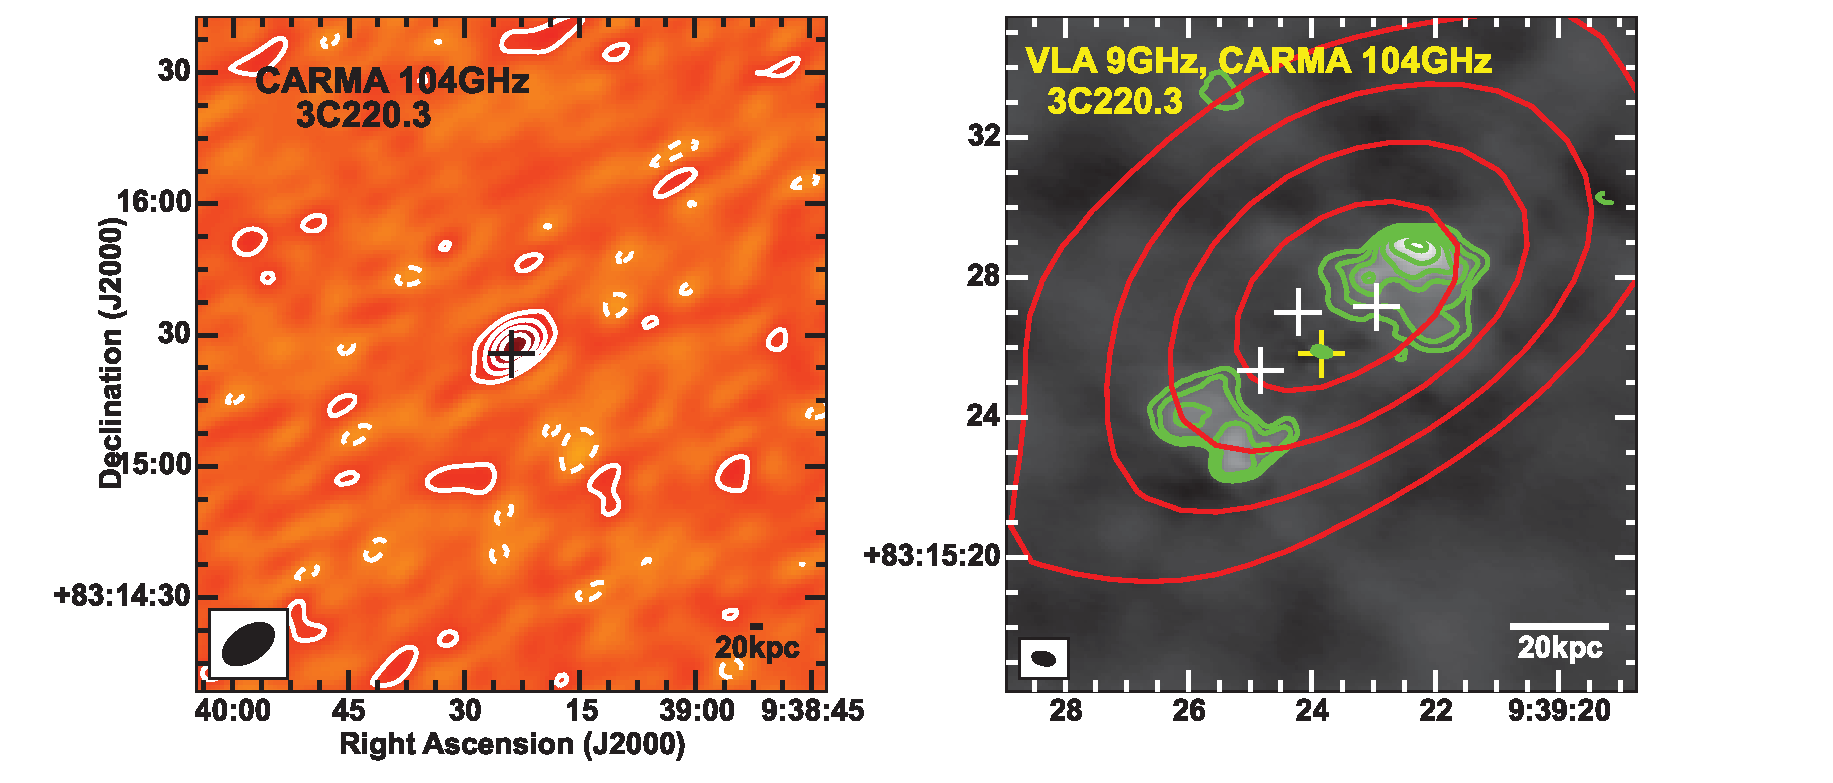
\includegraphics[width=0.80\textwidth]{Figure/ContPanel_cmyk.eps}
\caption{Left: Contour map of the 104 GHz continuum emission in the foreground radio galaxy 3C220.3.
%The contour levels start at $\pm$2$\sigma$, where $\sigma$ = 0.5 mJy beam\pmOne, and
%increment at steps of $\pm$2$\sigma$.
The beam size is 12\farcs0\,$\times$\,6\farcs5, at P.A.\,=\,
$-$56$\degr$, as indicated in the bottom left corner. Right: CARMA 104 GHz continuum emission (red contours) overlaid on the VLA 9 GHz continuum emission (green contours and grayscale; H14).
The synthesized beam size of the VLA observations is 0$\farcs$6\,$\times$\,0$\farcs$2, at P.A.
76$\degr$. The contour levels of the 104 GHz continuum emission start at $\pm$2$\sigma$, incrementing at steps
of $\pm$2$\sigma$, where $\sigma$ = 0.5 mJy beam\pmOne. The contour levels of the 9 GHz continuum
emission start at $\pm$4$\sigma$, where $\sigma$\,=\,0.064 mJy beam\pmOne, and increment at steps of $\pm$2$^n\sigma$,
where $n$ is a positive integer.
The central cross on each image indicates the position of the radio core of 3C220.3. \label{fig:cont}}
\end{figure*}
%\subsection{New Results: \CO Line Emission}
\subsection{New Results: SMM\,J0939\\ \CO Line Emission}
We detect \CO line emission at $\sim$\,8$\sigma$ significance toward the background SMG SMM\,J0939 at $z$\,=\,2.221.
The lensing-magnified spatial extent of this SMG is $\sim$\,5$\arcsec$, as shown in the Submillimeter Array (SMA) 1\,mm dust continuum image in Figure~\ref{fig:mom0} (H14); as such,
the detected \CO line emission is spatially unresolved. We therefore extract the line profile (Figure~\ref{fig:mom0}) at the peak position of the unresolved
CO emission. Fitting a four-parameter single Gaussian to the spectrum yields a peak flux density of 21.61\,$\pm$\,2.66\,\,mJy, superimposed on a
continuum level of 4.15\,$\pm$\,0.48~mJy~beam\pmOne, and a line full width at half-maximum (FWHM) of 546\,$\pm$\,36\,\,km\,\,s\pmOne.  \par
We construct a velocity-integrated (0$^\textrm{th}$ moment) map of the \CO line
emission after subtracting continuum emission in the visibility plane. This results in a velocity-integrated \CO line flux of $I_\textrm{CO}$\,=\,12.6\,$\pm$\,2.0 Jy km\,\,s\pmOne\ over a velocity range of $\Delta v$\,$\sim$\,1420 km\,\,s\pmOne, the uncertainty does not include $\sim$\,15\% calibration
uncertainty. Our \CO line measurement confirms the redshift of SMM\,J0939, yielding $z$\,=\,2.2212\,$\pm$\,0.0010.

\begin{figure*}[tbph]
\centering
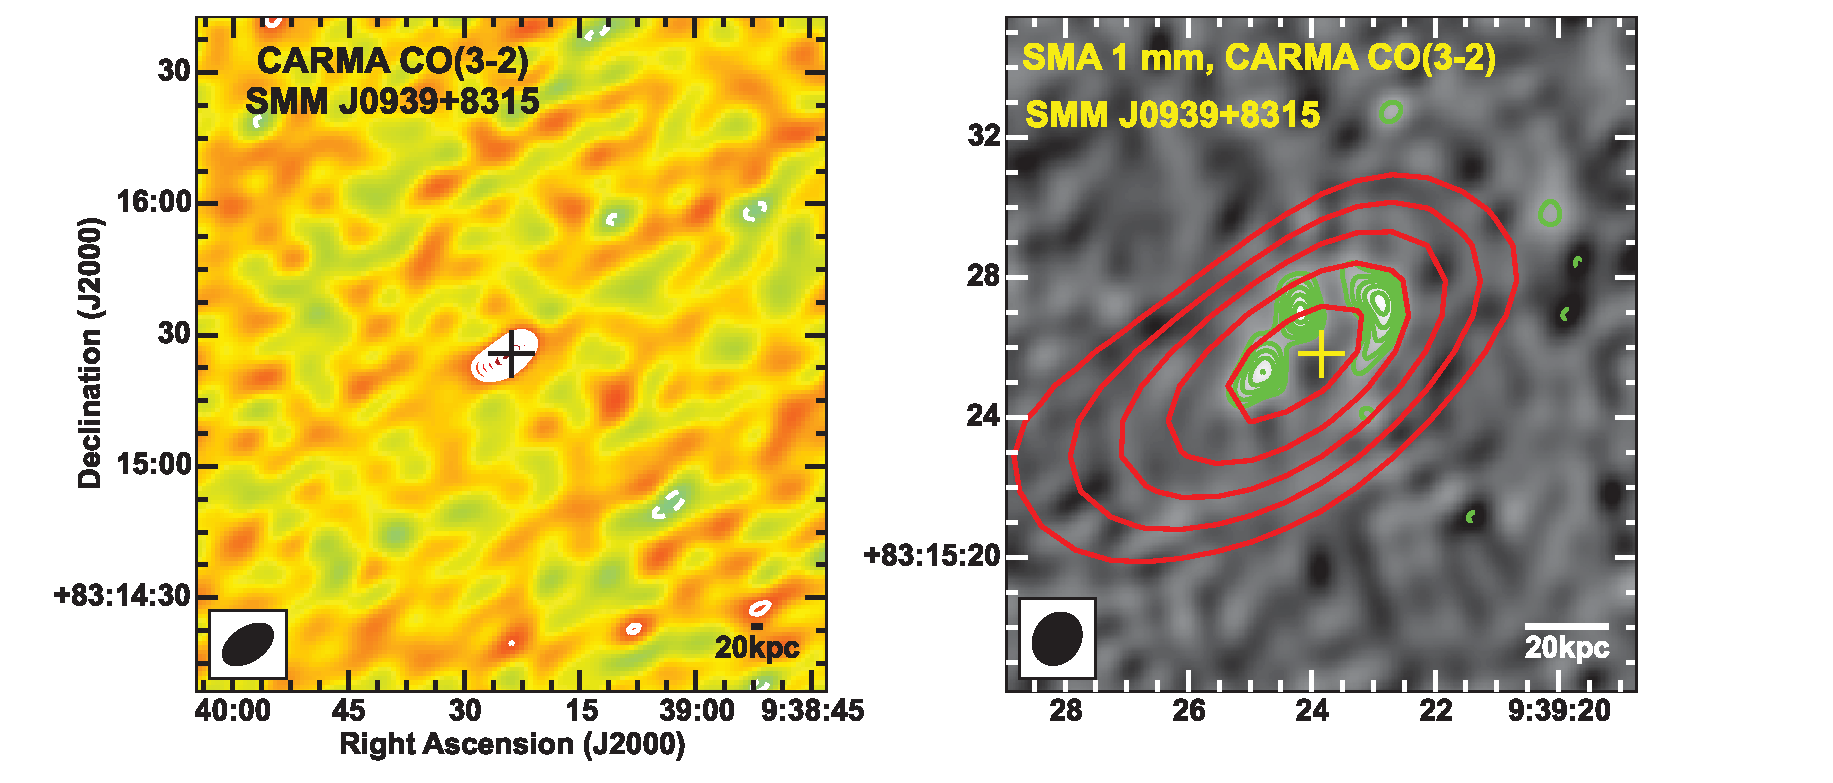
\includegraphics[width=0.8\textwidth]{Figure/LinePanel_cmyk.eps}
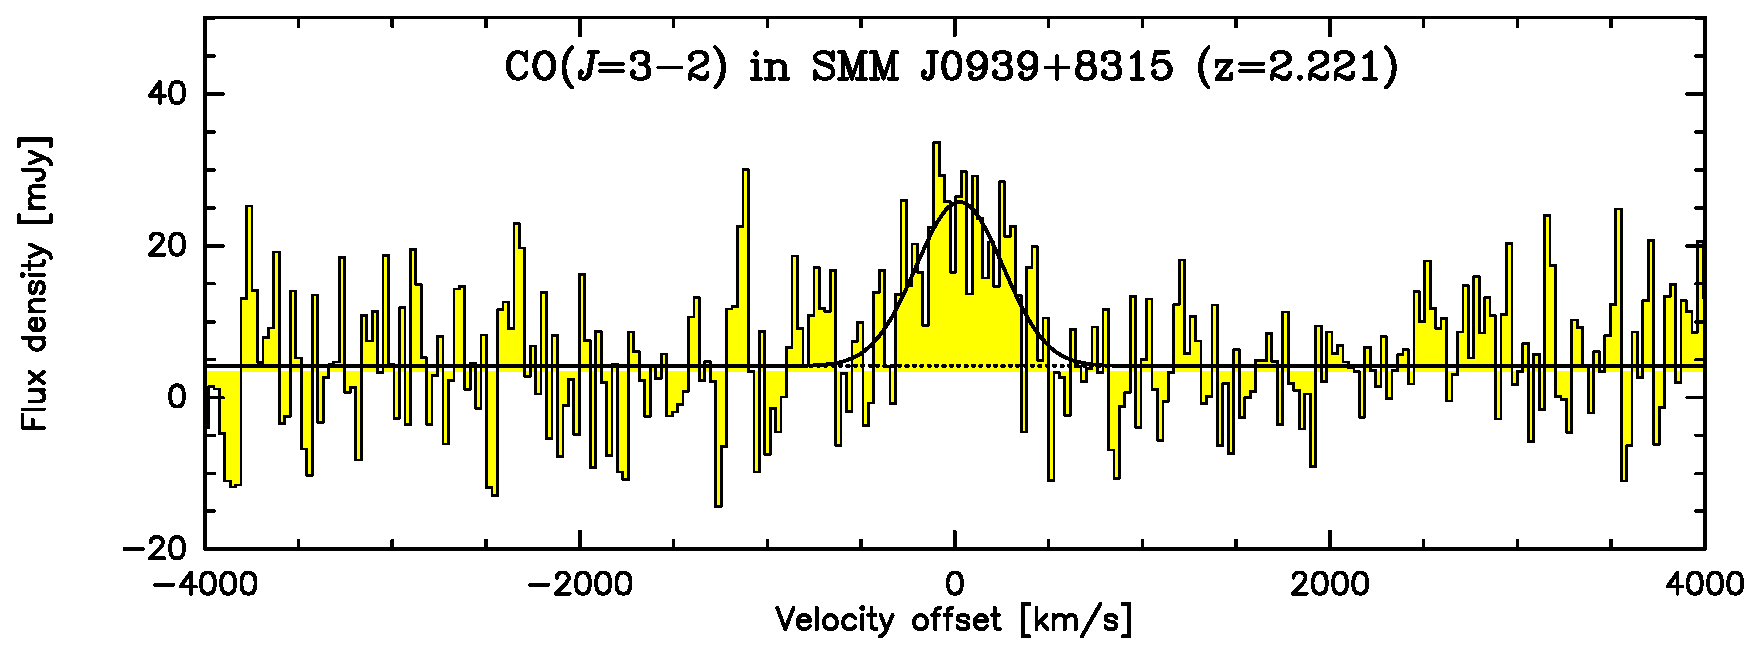
\includegraphics[width=0.65\textwidth]{Figure/smmj0939-co32_spec.eps}
\caption{Top Left: Continuum-subtracted moment-0 map of \CO line emission toward
the background SMG with $\sigma$\,=\,1.03\,Jy\,\,km\,\,s\pmOne\ beam\pmOne\ over a velocity range of $\Delta v$\,$\sim$\,514\,km\,\,s\pmOne. The beam size is 11$\farcs$5\,$\times$\,6\farcs2, at P.A.\,=\,$-$56\degr, as indicated in the bottom left corner.
Top Right: Velocity-integrated \CO line emission (red contours) overlaid on the SMA 1\,mm dust continuum (green contours and grayscale; H14), with an rms noise of $\sigma_\textrm{1\,mm}$\,=\,0.84 mJy beam\pmOne. The beam size of the SMA observations is 1\farcs4$ \times $1\farcs2, P.A. $-$34\degr, as shown
in the bottom left corner.
The central cross on each image corresponds to the same coordinates as in Figure~\ref{fig:cont}. The contour levels 
in both images
start at $\pm$3$\sigma$, incrementing at
steps of $\pm$1$\sigma$.
Bottom:
Spectrum extracted at the peak position of CO line emission, with a spectral resolution of $\Delta v$ $\sim$\,29 km\,\,s\pmOne, and an rms of $\sigma_\textrm{ch}$\,=\,9.5 mJy beam\pmOne\ per channel. The
solid black line shows a Gaussian fit to the \CO line profile, where the velocity scale is relative to $z$\,=\,2.221.
\label{fig:mom0}}
\end{figure*}


\section{Analysis}
\subsection{Lens Modelling} \label{sec:Lens}
To study the intrinsic properties of the background galaxy, we determine the magnification factor by performing
lens modeling on the SMA 1\,mm continuum data presented by H14 of this system. Lens modeling is carried out in the visibility
({\it uv-}) plane using the updated version\footnote{commit: 7aee6276} of the publicly available software {\sc uvmcmcfit}\footnote{\url{https://github.com/sbussmann/uvmcmcfit}}
\citep{Bussmann15a}. The code uses an affine-invariant Markov chain Monte Carlo (MCMC) approach to sample the posterior
probability density function (PDF) of the model parameters. In the code, the surface mass densities of both
lenses are represented by singular isothermal ellipsoid (SIE) profiles, and the source is assumed to have an
elliptical Gaussian profile. The code does not include an external shear parameter.

We fix the phase center to coordinates ($\alpha$,\,$\delta$)\,\,(J2000) = (9$^{\rm h}$39$^{\rm m}$23\fs54,\,\,83\degr15\arcmin26\farcs10), where the
angular offsets of the lenses and source are referenced to this position. The primary lens (3C220.3) is
described by five free parameters: the angular offset ($\Delta \alpha_{\rm
lens0}$ and $\Delta \delta_\textrm{lens0}$) relative to
the chosen phase center ($\alpha$,\,$\delta$) in the image, the angular Einstein radius ($\theta_\textrm{E0}$), the
axial ratio ($q_\textrm{lens0}$), and the position angle ($\phi_\textrm{lens0}$). The secondary lens (companion B) is
described by three free parameters: $\theta_\textrm{E1}$, $q_\textrm{lens1}$, and $\phi_\textrm{lens1}$. The angular offset
of the secondary
lens is sampled with respect to that of
the primary lens ($\Delta \alpha_\textrm{lens0}$ and $\Delta \delta_\textrm{lens0}$), we therefore do not consider ($\Delta \alpha_\textrm{lens1}$ and $\Delta \delta_\textrm{lens1}$)  as free parameters.
The source (SMM\,J0939) is parameterized by
six parameters: the position of the source relative to the
primary lens ($\Delta \alpha_\textrm{s}$ and $\Delta
\delta_\textrm{s}$), the total intrinsic flux density ($S_\nu$), the
effective radius ($r_\textrm{s}\,=\,\sqrt{a_\textrm{s} b_\textrm{s}}$), the axial
ratio ($q_\textrm{s}$\,=\, $b_\textrm{s}/a_\textrm{s}$), and the position angle
($\phi_\textrm{s}$).
%The total number of free parameters is $N_\textrm{free}$\,=\,14. 
The best-fit model is obtained by maximizing the
Gaussian likelihood function $ \mathcal{L} $ according to:
\begin{equation}
    \mathcal{L}\,=\,\sum_{u, v}\left( \frac{|V_\textrm{data} - V_{\rm
    model}|^2}{\sigma^2} + {\rm log}(2 \pi \sigma^2) \right)
\end{equation}
\noindent where $\sigma$ is determined from the scatter in the visibilities within a
single spectral window (``natural" weighting).

We initialize the positions and Einstein radii of both lenses, and the position of the source using those
 from the best-fit lens model performed on Keck K-band (near-infrared) data (H14). For each of
these parameters, we impose a uniform prior in the range $\in\pm$3$\sigma$, where $\sigma$ is the uncertainty
reported in their paper. The axial ratios of the lenses are restricted to $q_\textrm{lens} > 0.3$. We initialize 512
walkers and 6000 steps to identify the best-fit model parameters.
\begin{figure}[!tbpH]
\centering
\includegraphics[width=0.232\textwidth]{Figure/LensedSBmap_model_goodfit1970_cmyk}
\includegraphics[width=0.232\textwidth]{Figure/LensedSBmap_residual_goodfit1970_cmyk}
\caption{Double-lens modeling of SMM\,J0939 using {\sc uvmcmcfit} on the SMA 1\,mm continuum data.
The contours start at $\pm$2$\sigma$, incrementing at
steps of $\pm$2$\sqrt{\rm 2}\sigma$. Left: SMA 1\,mm continuum (red contours) overlaid on the best-fit model (grayscale image), assuming an elliptical Gaussian profile for the background SMG. The lenses are represented as black dots, the half-light area of the background source is represented as magenta ellipse, and the critical curves are represented as orange curves.
Right: Residual contours and image obtained by taking the Fourier transform of the difference between the SMA data and the best-fit model in the visibility plane. Solid (dashed) contours show the positive (negative) residuals.\label{fig:lens}}
\end{figure}

The resulting best-fit model as shown in Figure\,\,\ref{fig:lens} shows no significant bowls in the residual
image, and the knots (lensed emission) in the observed SMA data are well-reassembled with the best-fit model.
Our best-fit model yields a magnification
factor of $\mu_\textrm{L}$ = 10.13\,$\pm$\,1.38, this is consistent the value reported by H14 within the errors. All best-fit
parameters are listed in Table~\ref{tab:lensParam}. The Einstein radii associated with the best-fit model for the two lenses are $\theta_{E}$ = 1\farcs22\,$\pm$\,0\farcs01 (8.75 kpc at $z$\,=\,0.685) and $\theta_{E}$ = 0\farcs75\,$\pm$\,0\farcs02 (5.34\,\,kpc at $z$\,=\,0.685), and
the corresponding masses within the Einstein radii are $M(\theta$\,\,$<$\,\,$\theta_\textrm{E})$\,=\,(4.86\,$\pm$\,0.08)\,$\times$\,10$^{11}$\,\,\Msun\ and $M(\theta$\,\,$<$\,\,$\theta_\textrm{E})$\,=\,(1.82\,$\pm$\,0.07)\,$\times$\,10$^{11}$\,\,\Msun, respectively.
\begin{deluxetable}{l l r}[tbpH]
\tabletypesize{\scriptsize}
\tablecolumns{3}
\tablewidth{0pc}
\tablecaption{Lens modeling results}
\tablehead{
\multicolumn{2}{c}{Parameters} &
\colhead{Best-Fit Values}
\\ \cline{1-3} \vspace{-0.05in} \\
% \tableline
\multicolumn{3}{c}{Lens 0}
}
\startdata
%\cutinhead{Lens 0}
$\Delta \alpha_{\rm lens0}$      & (\arcsec)   & 0.403 $\pm$ 0.026     \\
$\Delta \delta_{\rm lens0}$      & (\arcsec)   & -0.181 $\pm$ 0.027    \\
$q_{\rm lens0}$ \tablenotemark{a} &             & 0.446 $\pm$ 0.063     \\
$\phi_{\rm lens0}$                & (deg)       & 31.56 $\pm$ 4.15\phn  \\
$\theta_{\rm E0}$                & (\arcsec)   & 1.218 $\pm$ 0.010     \\
\cutinhead{Lens 1}
$\Delta \alpha_{\rm lens1}$       & (\arcsec)   & -0.804 $\pm$ 0.034    \\
$\Delta \delta_{\rm lens1}$       & (\arcsec)   & -1.243 $\pm$ 0.017    \\
$q_{\rm lens1}$ \tablenotemark{a} &             & 0.608 $\pm$ 0.138     \\
$\phi_{\rm lens1}$                & (deg)       & 14.2 $\pm$ 15.7\phn      \\
$\theta_{\rm E1}$                & (\arcsec)   & 0.745 $\pm$ 0.015     \\
\cutinhead{Source}
$\Delta \alpha_{\rm s}$           & (\arcsec)   &  -0.163 $\pm$  0.035   \\
$\Delta \delta_{\rm s}$           & (\arcsec)   & -0.193 $\pm$  0.048   \\
$q_{\rm s}$ \tablenotemark{a}     &             & 0.424 $\pm$ 0.237     \\
$\phi_{\rm s}$                    & (deg)       & 174.34 $\pm$ 8.89\phn \\
$r$\tablenotemark{b}              & ($\arcsec$) & 0.106 $\pm$   0.033   \\
$\mu$                             &             & 10.13 $\pm$ 1.38\phn
\enddata
% 0.377 & -0.209 & 0.446 & 33.22 & 1.223 & -0.788 & -1.26 & 0.5289 & 9.55 & 0.733 & 9.74
\label{tab:lensParam}
\tablenotetext{a}{Axial ratio}
\tablenotetext{b}{Effective Radius}
% \tablenotetext{c}{}
\tablecomments{The angular offsets listed above are with respect to $\alpha$ = 9:39:23.54, $\delta$ = 83:15:26.10 (J2000). }
\end{deluxetable}

















\subsection{SED Fitting} \label{sec:SED}
\subsubsection{3C220.3}\label{sec:SEDFg}
Synchrotron continuum emission from extended components of a radio galaxy decreases with increasing radio frequencies,
and the spectrum is commonly characterized by a power law distribution $S \propto \nu^{-\alpha}$, where the
spectral index $\alpha$ is $\gtrsim$ 0.5. While the contribution from extended components decreases, studies using
samples of radio galaxies have suggested that the flat/inverted-spectrum of the compact radio core component rises
and dominates the flux density at higher frequencies \citep{Kellermann81a,Begelman84a}. This has been observed in a FR-II galaxy at similar redshift --- 3C220.1 at $z$ = 0.610, where observations were carried out at the observed-frame frequency of $\sim$\,90 GHz \citep{Hardcastle08a}.

Previously,  an upper
limit of $<$ 0.17 mJy at 4.6 GHz has been established by \citet{Mullin06a} on the core component of 3C220.3, and an unambiguous detection of 0.8 mJy at 9 GHz has been reported by H14, suggesting a substantially inverted spectrum of the core (Figure~\ref{fig:SED}).
Consequently, we may naively expect the integrated flux density in our continuum detection of $S_\textrm{104GHz}$\,=\,7.39\,$\pm$\,1.42\,\,mJy to be dominated by the unresolved core component of the foreground FR-II galaxy, which is at $z$\,=\,0.685.
However, the deconvolved spatial size of the source matching that in the resolved image (see Figure~\ref{fig:cont}) is
suggestive of a marginally resolved detection of the extended lobe components with non-negligible emission.
This is plausible given that the orientation of the synthesized beam in our observations is in alignment with the
axis along the
lobes of the radio galaxy, as shown in Figure~\ref{fig:cont}. We investigate this disparity by fitting models to
existing SED measurements as listed in Table \ref{tab:SEDdataRadio}, and extrapolating the fit to
estimate the flux density of the lobes at the frequency of our continuum measurement.
\begin{deluxetable}{rlrcc}[tbpH]
\tabletypesize{\scriptsize}
\tablecolumns{5}
\tablecaption{Continuum data of 3C220.3}
\tablehead{
\multicolumn{2}{c}{Frequency} &
\multicolumn{2}{c}{Flux Density} &
\colhead{Reference} \vspace{0.05in}
\\  \cline{1-5} \vspace{-0.05in} \\
\multicolumn{5}{c}{Integrated (Core \& Lobes)}
}
\startdata
    104.2 & GHz & 7.39 $\pm$ 1.42\tna        & mJy & LR15 \\
%    104.2 & GHz & 4.91 $\pm$ 0.54\tna        & mJy & This work \\
    10.7  & GHz & 270 $\pm$ 30            & mJy & KP73       \\
    10.7  & GHz & 253 $\pm$ 28            & mJy & L80       \\
    5.0   & GHz & 640 $\pm$ 100           & mJy & K69       \\
    5.0   & GHz & 636 $\pm$ 50            & mJy & L80       \\
    2.7   & GHz & 1.33 $\pm$ 0.07         & Jy  & K69       \\
    2.7   & GHz & 1.34 $\pm$ 0.10         & Jy  & L80       \\
    1.4   & GHz & 2.95 $\pm$ 0.09         & Jy  & C98       \\
    1.4   & GHz & 2.99 $\pm$ 0.06         & Jy  & P66       \\
    1.4   & GHz & 2.80 $\pm$ 0.14         & Jy  & K69       \\
    1.4   & GHz & 2.89 $\pm$ 0.09         & Jy  & L80       \\
    0.75  & GHz & 5.94 $\pm$ 0.28         & Jy  & L80       \\
    0.75  & GHz & 5.94 $\pm$ 0.21         & Jy  & P66       \\
    0.75  & GHz & 5.60 $\pm$ 0.84         & Jy  & K69       \\
    352   & MHz & 11.3 $\pm$ 0.453        & Jy  & WENSS     \\
    352   & MHz & 11.6 $\pm$ 0.464        & Jy  & WENSS     \\
    178   & MHz & 15.7 $\pm$ 2.35         & Jy  & K69       \\
    178   & MHz & 17.1 $\pm$ 1.71         & Jy  & L80       \\
    152   & MHz & 22.6 $\pm$ 0.08         & Jy  & B85       \\
    152   & MHz & 22.5 $\pm$ 0.04         & Jy  & B85       \\
    86    & MHz & 51.6 $\pm$ 9.90         & Jy  & L80       \\
    73.8  & MHz & 37.5 $\pm$ 3.82         & Jy  & C07       \\
    38    & MHz & 49.6 $\pm$ 4.96         & Jy  & L80       \\
    38    & MHz & 40.2 $\pm$ 6.30         & Jy  & K69       \\
    37.8  & MHz & 60.7 $\pm$ 6.07         & Jy  & H95       \\
    17.8  & MHz & 64.9 $\pm$ 6.49         & Jy  & H95			\\
\cutinhead{Core Only}
    104.2 & GHz & $<$ 2.29 		      & mJy & LR15 \\
    9.0   & GHz & 0.80  $\pm$ 0.06    & mJy & H14       \\
    4.86  & GHz & $<$ 0.17            & mJy & M06       \\
\enddata
\label{tab:SEDdataRadio}
\tablenotetext{a}{Integrated flux density. Peak flux density of the continuum emission is 4.93 $\pm$ 0.31 mJy beam\pmOne}
%\tablenotetext{b}{Core only}
\tablenotetext{$\dagger$}{www.astron.nl/wow/testcode.php?survey=1}
%\tablecomments{References.~}
\tablerefs{
B85 = \citet{r2728};
C98 = \citet{r16};
C07 = \citet{r30};
H95 = \citet{r33-34};
H14 = \citet{Haas14};
K69 = \citet{r11-14-18-22-25-32};
KP73 = \citet{r9};
L80 = \citet{r10-13-15-19-20-26-29-31};
LR15 = this work;
M06 = \citet{Mullin06a};
P66 = \citet{r17-21};
WENSS = \citet{r23-24}$^\dagger$
}
\end{deluxetable}
















Following Equation (1) in \citet{Cleary07a}, the fit to the lobe emission can be expressed as a parabolic function:
\begin{equation}
\log F_{\nu}^{\mathrm lobe} (\nu) \propto - \beta\ (\log\ \nu - \log \nu_{t})^2  + \log (\exp({\frac{\nu}{\nu_c^{\mathrm lobe}}}))
\end{equation}
where $F_{\nu}^{\mathrm lobe}$ is the flux density of the lobes, $\beta$ is a parameter representing the bending
of the parabola, $\nu_t$ is the frequency at which the optical depth of the synchrotron emitting plasma reaches
unity, and $\nu_c^{\rm lobe}$ is the frequency corresponding to the cutoff energy of the lobe plasma energy
distribution. 
The extrapolated flux density at 104\,\,GHz is consistent with the peak flux density of our continuum
measurement (Figure~\ref{fig:SED}). The 9$\sigma$ detection of the continuum thereby suggests a
dominant contribution from the lobes, and that the peak flux density does not correspond to emission toward
the core. Moreover, the peak position of the 104\,\,GHz continuum is
centered toward the northern lobe (Figure~\ref{fig:cont}), which further supports our argument. 
Consequently, a conservative upper limit of $S_\nu$\,$<$\,4.93 mJy on the core emission can be established using the measured peak flux density. Yet, by considering the 
difference between the integrated flux density from our measurement and the flux density from an extrapolation of the model (see Figure~\ref{fig:SED}; $S_\textrm{104GHz, fit}$~=~5.10 mJy), we establish a more stringent constrain on this upper limit of $S_\nu$\,$<$\,2.29 mJy. We did not 
 extrapolate the core measurements to the frequency of our continuum, as previous measurements of the core are 
 taken 
 across different epochs. 
\par
Studies by \citet{Meisenheimer89a} and \citet{Hardcastle08a} have suggested that spectra of hotspots are flat up to optical frequencies, where some exhibit spectral steepening in cm and mm wavelengths (\eg 3C123). At the resolution of our observations, it is unclear whether the measured flux density is dominated by emission from the compact hotspot or that from the surrounding diffuse lobe components.

\begin{figure}[!tbph]
\centering
\includegraphics[width=0.5\textwidth]{Figure/3C220_3_FullSED2}
\caption{SEDs of 3C220.3 (solid purple line) and SMM\,J0939 (dashed purple line and solid cyan line) including the new measurements presented in this paper.
The solid purple line corresponds to the parabolic function we
fit to the existing data associated with 3C220.3 (black dots; see Table \ref{tab:SEDdataRadio}).
The red dots at 104 GHz correspond to
our continuum measurements (integrated, peak, and difference, respectively).
The dashed purple line and
the solid cyan line correspond to the best-fit optically thick and optically thin models of SMM\,J0939, respectively, using the photometric data from H14. \label{fig:SED}}
\end{figure}

\subsubsection{SMM\,J0939+8315} \label{sec:SEDBg}
To constrain the dust and gas properties in the ISM of SMM\,J0939, we perform SED fitting to the
photometric data obtained with {\it Herschel}/PACS and SPIRE, at wavelengths
between observed-frame 70\,\micron\,$-$\,500\,\micron, and the interferometric data obtained with the SMA at 1\,mm (H14). We use the publicly
available software {\sc mbb\_emcee}\footnote{\url{https://github.com/aconley/mbb\_emcee}} to perform the SED fitting; the code uses an affine-invariant Markov chain Monte
Carlo (MCMC) approach, and further details of the code are given by \citet{Riechers13a} and \citet{Dowell14a}. \par
The
functional form of the fit comprises a single-temperature, modified blackbody function joined to a $S_{\lambda} \propto \lambda^\alpha
$ power law on the blue
side of the SED.
We fit both optically thick and optically thin models. In the optically thick case, the wavelength $
\lambda_0$\,=\,${c}/{\nu_0}$ is an additional parameter representing the rest-frame wavelength at which the optical
depth $\tau_{\nu} =$ ($\nu$/$\nu_0$)$^\beta$ reaches unity. Thus, the functional form of the modified blackbody
in the optically thick regime is as follows:
\begin{equation}
\rm S_{\lambda} \propto \frac{(1-exp^{-(\frac{\lambda_0 (1+z)}{\lambda})^{\beta}})(\frac{c}{\lambda})^3}
{exp^{\frac{hc}{\lambda\rm{kT/(1+z)} } }-1}
\end{equation}
and in the optically thin regime, the functional form reduces to:
\begin{equation}
\rm S_{\lambda} \propto \frac{(\frac{c}{\lambda})^{\beta+3}}{exp^{\frac{hc}{\lambda\rm{kT/(1+z)}}}-1}
\end{equation}
where $T$ is the rest-frame cold dust temperature, $\beta$ is the dust emissivity index 
%(equivalently, the spectral index of the dust extinction curve)
, and $\alpha$ is the mid-infrared power law spectral index. The overall fit is normalized using the observed-frame 500
$\micron$ flux density, hence this becomes an additional parameter in the fit. For both models, we impose an upper limit of 60 K on the observed-frame dust temperature ($T/(1+z)$), an upper limit of 2.2 on
$\beta$. For the optically thick model, we impose an additional upper limit of 2000\,\micron\ on $\lambda_0$.

\begin{deluxetable}{ccc}[tbpH]
\tabletypesize{\scriptsize}
\tablecolumns{3}
\tablecaption{SED fitting results}
\tablehead{
\colhead{Parameters}                  &
\colhead{Optically Thick}       &
\colhead{Optically Thin}
}
\startdata
$\chi^2$ & 2.25 & 5.31 \\
D.O.F & 2 & 3 \\
$T_{\rm d}$ (K) & 60.91$^{+1.08}_{-1.31}$ & 51.95$^{+1.26}_{-1.21}$ \\
$\beta$ & 1.35$^{+0.57}_{-0.53}$ & 0.7$^{+0.24}_{-0.26}$ \\
$\alpha$ & 3.05$^{+0.31}_{-0.40}$ & 2.76$^{+0.23}_{-0.23}$ \\
%$\lambda_0$(1+$z$) ($\micron$) \tablenotemark{c} & 722.81$^{+276.88}_{-398.67}$ & --- \\
$\lambda_0$ ($\micron$) \tablenotemark{e} & 224.41$^{+85.96}_{-123.77}$ & --- \\
$\lambda_{\rm peak}$ \tablenotemark{c}\micron & 254.7$^{+6.2}_{-6.1}$ & 301.4$^{+29.0}_{-30.1}$ \\
$f_{\rm norm, 500 \micron}$ mJy  \tablenotemark{c} & 255.79$^{+16.67}_{-16.31}$ & 244.25$^{15.28}_{15.30}$ \\
$L_{\rm (8-1000)\micron}$ [10$^{12}$ L$_\sun$] \tablenotemark{d} & 88.52$^{+2.62}_{-2.63}$ & 89.15 \\
$M_{\rm d}$ [10$^8$ M$_\odot$] \tablenotemark{b} & 50.47$^{+20.42}_{-20.15}$ & 25.74$^{+3.88}_{-5.49}$
\enddata

% Optically thick & 18.91 & 1.35 & 722.81 & 3.05 & 254.7 & 88.52 & 50.47 \\
% Optically thin &  16.13 & 0.7 & N/A   & 2.76 & 301.4 & 89.15 & 25.74

\label{tab:mbb}
\tablenotetext{a}{The observed-frame wavelength where the dust becomes optically thick}
\tablenotetext{b}{Assuming standard absorption mass coefficient $\kappa$=2.64 m$^2$ kg$^{-1}$ at $\lambda$=125.0 $\micron$ (Dunne et al. 2003), without lensing correction}
\tablenotetext{c}{observed-frame}
\tablenotetext{d}{rest-frame 8-1000 $\micron$ without lensing correction}
\tablenotetext{e}{The rest-frame wavelength where the dust becomes optically thick, upper limit is 2000 $\micron$}
\tablecomments{Errors are $\pm$1$\sigma$}
\end{deluxetable}

% thick_500_500.log
% T/(1+z): 18.91 +1.09 -1.31 (low lim: 1.00 upper lim: 60.00) [K]
% beta: 1.35 +0.57 -0.53 (low lim: 0.10 upper lim: 2.20)
% fnorm: 255.79 +16.67 -16.31 (low lim: 0.03) [mJy]
% lambda0 (1+z): 722.81 +276.88 -398.67 (low lim: 1.00 upper lim: 3049.15) [um]
% alpha: 3.05 +0.31 -0.40 (low lim: 0.10 upper lim: 20.00)
% Lambda peak: 254.7 +6.2 -6.1 [um]
% L_IR(8.0 to 1000.0um): 88.52 +2.62 -2.63 [10^12 L_sun]
% M_d(kappa=2.64, lam=125.0um): 50.47 +20.42 -20.15 [10^8 M_sun]
% Number of data points: 7
% ChiSquare of best fit point: 2.25

% note using beta upper limit 3.0, getting very different beta, and dust mass
% Fit results:
% T/(1+z): 19.75 +0.56 -0.53 (low lim: 1.00 upper lim: 60.00) [K]
% beta: 1.91 +0.76 -0.76 (low lim: 0.10 upper lim: 3.00)
% fnorm: 267.13 +16.03 -15.98 (low lim: 0.03) [mJy]
% lambda0 (1+z): 1012.99 +142.79 -275.29 (low lim: 1.00 upper lim: 3049.15) [um]
% alpha: 3.64 +0.08 -0.86 (low lim: 0.10 upper lim: 20.00)
% Lambda peak: 255.6 +6.3 -6.2 [um]
% L_IR(8.0 to 1000.0um): 88.02 +2.85 -2.85 [10^12 L_sun]
% M_d(kappa=2.64, lam=125.0um): 108.23 +32.00 -63.67 [10^8 M_sun]
% Number of data points: 7
% ChiSquare of best fit point: 2.25
% Saving results to thick_testbeta.h5

% thin_testSMA
% T/(1+z): 16.13 +1.26 -1.21 (low lim: 1.00 upper lim: 60.00) [K]
% beta: 0.70 +0.24 -0.26 (low lim: 0.10 upper lim: 3.00)
% fnorm: 244.25 +15.28 -15.30 (low lim: 0.03) [mJy]
% alpha: 2.76 +0.23 -0.23 (low lim: 0.10 upper lim: 20.00)
% Lambda peak: 301.4 +29.0 -30.1 [um]
% L_IR(8.0 to 1000.0um): 89.15 +2.48 -2.51 [10^12 L_sun]
% M_d(kappa=2.64, lam=125.0um): 25.74 +3.88 -5.49 [10^8 M_sun]
% Number of data points: 7
% ChiSquare of best fit point: 5.31

The best-fit values in both regimes are listed in Table \ref{tab:mbb}, and the correlation plots are available in the Appendix. The best-fit solution of an optically thin
model corresponds to $\chi^2$ = 5.31 with 3 degrees of freedom, whereas that of an optically thick model
corresponds to $\chi^2$ = 2.25 with 2 degrees of freedom, suggesting a better fit than in the optically thin
case. In the subsequent analysis, we employ the inferred values from the optically thick model.
The best-fit solution yields a FIR luminosity (rest-frame 42.5$-$122.5\micron) of $L_\textrm{FIR}$ = 53.3$^{+1.1}_{-1.1}$\,$\times$\,10$^{12}$\,\Lsun, and a total infrared (IR; rest-frame 8$-$1000 \micron) luminosity of $L_\textrm{IR}$ = 88.5$^{+2.6}_{-2.6}$\,$\times$\,10$
^{12}$\,\Lsun. Assuming a dust absorption coefficient of $\kappa_{\nu}$ = 2.64\,\,m$^2$\,\,kg\pmOne\ at 125.0\,\,$
\micron$ \citep{Dunne03a}, we derive the dust mass using the following expression:
\begin{equation}
M_\textrm{dust}\,=\,S_{\nu} D_{L}^2 [(1 + z) \kappa_{\nu} B_{\nu}]^{-1} \tau_{\nu} [1-
\exp(-\tau_{\nu})]^{-1}
\end{equation}
where $S_{\nu}$ is the flux density in erg\,s\pmOne\,cm$^{-2}$\,Hz\pmOne, $D_\textrm{L}$ is the luminosity distance in cm, $\kappa_{\nu}$ is the dust
absorption coefficient in cm$^2$\,g\pmOne, $\tau_{\nu}$ is the optical depth, and $B_{\nu}$ is the Planck function in units of erg\,s\pmOne\,cm$^{-2}$\,Hz\pmOne\,sr\pmOne;
all quantities are expressed in the observed-frame. We find a dust mass of $M_\textrm{dust}$ = 50.5$^{20.4}_{-20.2}\times$10$^8$\,\,\Msun, the uncertainties do not include those in the dust absorption coefficient ($\kappa_{\nu}$). These properties are derived based on the SED fitting to the photometric data, \ie prior
to lensing correction.

With the limited amount of data in the FIR waveband, the dust mass is weakly constrained.
We perform an additional fit using an optically thick model where we loosen the upper limit of $\beta$ from 2.2 to 3.0; while the difference between each of all best-fit parameters in this scenario and that using an upper limit of 2.2 is within 3\%, we find that the dust mass is boosted by a factor of $\sim$\,2.
\subsection{Physical Properties of the ISM in SMM\,J0939}
\subsubsection{Molecular Gas Mass}
While the ground state CO transition line traces the cold molecular gas in the ISM
\citep*[\eg][]{Wilson70a,Downes98a}, transition lines of higher rotational states ($J$ $>$ 1) are frequently observed in high-redshift sources as the
 ground state transition line is redshifted to lower frequencies that can only be observed with a few telescopes
 \citep{Carilli13a}. Consequently, assumptions on the CO excitation conditions are required to derive the molecular gas mass using the M(H$_\textrm{2}$)-to-$L^{\prime}_\textrm{CO}$
 conversion factor from higher-$J$ CO lines. \par
Prior to the observations of the ground state CO transition line in SMGs, it had been assumed that the molecular gas in the
  ISM traceable by CO lines was thermalized owing to their high star formation rates \citep[\eg][]{Greve05a, Coppin08a}.
   Yet, recent observations of this line have demonstrated that SMGs can indeed be subthermally excited
   \citep{Harris10a,Riechers11c,Riechers11d,Ivison11a}. Namely, observational results of SMGs with both \CO and CO($J$\,=\,1\,\rarr\,0) line measurements have shown that the
   brightness temperature ratio is more commonly found to be $R_\textrm{31}<$ 0.8 \citep
   {Harris10a,Carilli10a,Swinbank2010a,Ivison10d,Ivison11a,Riechers11d}. In contrast, similar observations in high-redshift quasar hosts suggest that the ratio
   is $R_\textrm{31}$\,$\sim$\,1 \citep{Riechers06a, Riechers11a}. In the case of high-redshift type-2 quasars, \citet{Riechers11a} report a brightness temperature ratio of $R_\textrm{31}$ = 1.00\,$\pm$\,0.10 for IRAS F10214+4724 (hereafter F10214), which is currently the only known type-2 quasar with both \CO and CO($J$\,=\,1\,\rarr\,0) line measurements. \par
Here, we derive the molecular gas mass
assuming thermalized excitation of CO,
\ie we adopt $R_\textrm{31}$\,=\,1, as SMM\,J0939 is
postulated to be hosting a type-2 quasar (H14).
We calculate the CO($J$\,=\,1\rarr\,0) line luminosity using standard relation
\citep[\eg][]{Solomon05a,Carilli13a}:
\begin{equation}
L^{\prime}_\textrm{CO}\,=\,\frac{3.25\times10^7}{\nu_\textrm{CO(3-2)}^2}\times \frac{D_L^2}{\mu_\textrm{L}} \times
\frac{I_\textrm{CO(3-2)}} {R_\textrm{31} (1 + z)}
\end{equation}
where $\nu_\textrm{CO(3-2)}$ is the rest-frame frequency of the \CO transition line in GHz, $D_L$ is the luminosity distance in Mpc, $\mu_\textrm{L}$ is the lensing magnification factor, and $I_\textrm{CO(3-2)}$ is the \CO line flux in Jy\,\,km\,\,s\pmOne. This corresponds to \Lp = (3.42\,$\pm$\,0.71)\,$\times$~10$^{10}$\,(10.1/$\mu_\textrm{L}$)~\LpU, hence
the inferred total molecular gas mass is $M_\textrm{gas}$ = (2.74\,$\pm$\,0.57)\,$\times$\,\,10$^{10}$\,\Msun\, after correcting for lensing magnification. We assumed a conversion factor of $\alpha_\textrm{CO}$ = 0.8\,\,\Msun\,(\LpU)\pmOne\ based on empirical relations from local ULIRGs, which is typically
adopted for SMGs \citep[\eg][]{Tacconi06a,Tacconi08a,Bothwell13a}.
This results in a gas-to-dust
ratio of $f_\textrm{gas-dust}$\,=\,$M_\textrm{gas}/M_\textrm{dust}$\,=\,55\,$\pm$\,24. We note that a factor of $\sim$\,2 uncertainty arises from the dust mass estimate. The derived gas-to-dust ratio is in good agreement, within the uncertainties, 
 with the
values found in other SMGs \citep{Coppin08a,Micha10a,Riechers11c}.

\subsubsection{Star Formation Rate}
%No strong evidence of a hot dust bump is found in SMM\,J0939 based on the mid-IR (WAIT, BUT ONLY HAVE 70 micron onwards) continuum measurements (see Figure~\ref{fig:SED}), hence
We derive the star formation rate (SFR) assuming that the dominant IR heating source is due to young and massive stars, and ignoring a contribution from the
dust-enshrouded AGN.
Using the \citet{Kennicutt98a} relation and assuming a \citet{Chabrier03a}
stellar initial mass (IMF) function\footnote{The SFR would be SFR$_\textrm{FIR}$\,=\,526\,$\pm$\,73 $M_
\odot$ yr\pmOne\ if we were to use only the FIR luminosity},
we derive a SFR$_\textrm{IR}$ of 874\,$\pm$\,122 $M\sun$\,\,yr\pmOne, employing the lensing-corrected total IR luminosity.
The starburst in SMM\,J0939 can be maintained at its
current rate for a time that can be approximated by the gas depletion timescale, $\tau_\textrm{depl}$\,=\,$M_\textrm{gas}$/SFR.
This corresponds to $\tau_\textrm{depl}$\,=\,31\,$\pm$\,5 Myr, which is in good agreement with those found in other SMGs \citep[\eg][]{Greve05a}.

\subsubsection{Star Formation Efficiency}
The SFR per unit mass of molecular gas is commonly taken as a
measure of the star formation efficiency, SFE\,=\,SFR/$M_\textrm{gas}$. We compute this ratio using the IR
luminosity and CO luminosity without correcting for lensing magnification, SFE\,=\,$L_\textrm{IR}$/\Lp. The derived SFE is therefore independent of the magnification factor, the CO luminosity to gas mass conversion factor ($\alpha_\textrm{CO}$), and of the
IMF. This, however, assumes that differential lensing between the CO and infrared emission is negligible.
The resulting ratio is SFE$_\textrm{IR}$\,=\,256\,$\pm$\,41\,\,\Lsun\,(\LpU)$^{-1}$, this is comparable
to those found in ``typical" SMGs \citep{Greve05a,Tacconi06a,Riechers11c}.

\subsubsection{Dynamical Mass}
Based on our \CO line measurement, we estimate the dynamical mass of SMM\,J0939 assuming that the molecular gas is virialized. With this assumption, we use an isotropic virial estimator \citep[\eg][]{Engel10a}:
\begin{equation}
M_\textrm{dyn}\,=\,2.8\times 10^5\Delta v_\textrm{line}^ 2 R_\textrm{eff}
\end{equation}
where $\Delta v_\textrm{line}$ is in km\,\,s\pmOne, $R_\textrm{eff}$ is in kpc, and $M_\textrm{dyn}$ is in \Msun.
We employ the FWHM of the \CO line profile for $\Delta v_\textrm{line}$,
and the half-light radius from our lens model for $R_\textrm{eff}$, assuming that the dust emission traces the same emitting region as the CO. We note that a derived dynamical mass based on this assumption is likely to be biased low as the CO-emitting region can be spatially more extended than the dust emitting region \citep[\eg][]{Tacconi06a, Riechers11c,Riechers11d,Ivison11a}.
% 
The inferred dynamical mass is $M_\textrm{dyn}$ = (7.84\,$\pm$\,2.84)\,$\times$\,10$^{10}$\,\Msun, and the gas-to-dynamical mass fraction is $f_\textrm{gas-to-dyn}$ = 0.35\,$\pm$\,0.14, consistent with those of other SMGs \citep{Tacconi06a}.

\subsubsection{Star Formation and Gas Surface Densities}
To compute surface densities, we divide half the inferred SFR and gas mass by the area subtended by the half-light
radius, resulting in $\Sigma_\textrm{gas}$ = 5.48\,$\times$\,10$^9$ \Msun~kpc$^{-2}$ and $\Sigma_\textrm{SF}$ = 175.20 \Msun~yr\pmOne~kpc$^{-2}$, which are in good agreement with values typical for SMGs \citep{Tacconi08a}. 
The inferred surface densities of SMM\,J0939 follow a universal Schmidt-Kennicutt relation between the star formation rate
surface density and the molecular gas surface density: $\Sigma_\textrm{SF}$ = 9.3 ($\pm$\,2)\,$\times$\,10$^{-5}$ ($M_\textrm{gas}$/2$\pi R_\textrm{1/2}^2)^{1.71(\pm\,0.05)}$, which was derived using a sample consisting of local star-forming galaxies and high-redshift
galaxies
out to $z$\,$\sim$\,2.5, and assuming a Chabrier IMF \citep{B07a}.

\section{Discussion And Conclusions}
\newcommand\tnh{\,\tablenotemark{h}}
\newcommand\tni{\,\tablenotemark{i}}
\newcommand\tnj{\,\tablenotemark{j}}
\newcommand\tnk{\,\tablenotemark{k}}
\begin{deluxetable*}{l l c c c c c}[tbpH]
\tabletypesize{\scriptsize}
\tablecolumns{7}
\tablecaption{Comparison of SMM J0939 with SMGs at $z\sim$2}
\tablehead{
\multicolumn{2}{c}{SMGs}       &
\colhead{SMM J0939}  &
\multicolumn{2}{c}{HLSW-01}    &  
\multicolumn{2}{c}{Cosmic Eyelash} 
                     \\
\colhead{Quantity} &
\colhead{Unit} &
\colhead{}                     &
\colhead{}                     &
\colhead{Ref.}                     &
\colhead{}                     &
\colhead{Ref.}
}
\startdata
$z$             &                   & 2.221            & 2.957            & R11              & 2.326          &  S10 \\
$\mu_{\rm L}$         &                   & 10.1 $\pm$ 1.4    & 10.9 $\pm$ 0.7 & G11              & 37.5$\pm$4.5    &  S11 \\
$S_{\rm 250}$ & mJy & 440 $\pm$15 (H14) & 420 $\pm$ 10  & R11              & 366 $\pm$ 55  & I10             \\
$I$\tnb       & Jy km s$^{-1}$   & 10.7 $\pm$ 2.1   & 9.7 $\pm$ 0.5  & R11              & 13.2 $\pm$ 0.1 &  D11 \\
$\Delta v_{\rm FWHM}$\tnb & km s$^{-1}$ & 542 $\pm$ 32 & 350 $\pm$ 25 & R11 & $\lesssim$ 800\tnd & D11 \\
\Lp & 10$^{10}$ \LpU & 2.91 $\pm$ 0.78\tnh & 4.17 $\pm$ 0.41 & R11 & 1.7 $\pm$ 0.2 & D11 \\
$M_{\rm gas}$ & 10$^{10}$ \Msun & 2.33 $\pm$ 0.62\tnh & 3.3 $\pm$ 0.3 & R11 & 1.6 $\pm$ 0.1 & I10 \\
$L_{\rm IR}$ &  10$^{12}$ \Lsun & 9.1 $\pm$ 1.2\tnh & 14.3 $\pm$ 0.9 & C11 & 2.3 $\pm$ 0.2 & I10 \\
$M_{\rm dust}$ & 10$^8$ \Msun & 5.2 $\pm$ 2.1\tnh  & 1 - 5.2
& R11 & $\sim$4.0 & I10 \\
SFR$_{\rm IR}$\tna & \Msun yr$^{-1}$ & 874 $\pm$ 122\tnh & 1430 $\pm$ 160\tnc & C11 & $\sim$235\tnc & I10 \\
$\tau_{\rm depl}$\tng & Myr & 25.6 $\pm$ 0.6 & 23 $\pm$ 3\tnc  & R11 & 68\tne & --- \\
$f_{\rm gas-dust}$\tng &  & 47 $\pm$ 21 & 60-330 & R11 & $\sim$ 40 & I10 \\
SFE\tng  & Myr$^{-1}$ & 300 $\pm$ 10 & 340 $\pm$ 40 & R11 & 165 $\pm$ 7 & D11 \\
$M_{\rm dyn}$\tng & 10$^{10}$ \Msun & 7.4 $\pm$ 2.4 & 3.7 $\pm$ 1.8\tne\tnf & --- & 6.0$\pm$0.5 & S11 \\
$f_{\rm gas-dyn}$ && 0.32$\pm$0.14 & 0.90\tne\tnf & --- & 0.6$\pm$0.1 & S11 \\
\enddata
\label{tab:comapreSMG}
\tablenotetext{a}{Chabrier IMF}
\tablenotetext{b}{\CO}
\tablenotetext{c}{Converted theirs values derived using Salpeter IMF to Chabrier IMF}
\tablenotetext{d}{Estimated from Figure 1 in D11}
\tablenotetext{e}{We derive this using the reported values}
\tablenotetext{f}{Using CO($J$ = 5 \rarr\ 4)}
\tablenotetext{g}{Independent of lensing magnification factor $\mu_{\rm L}$}
\tablenotetext{h}{Errors include uncertainties on $\mu_{\rm L}$}
%\tablenotetext{i}{Based on 1 mm continuum}
%\tablenotetext{j}{Based on }
%\tablenotetext{k}{Based on 870 micron, CO 1-0, 6-5, and HST}
%\tablenotetext{f}{Using $L_{\rm IR} / M_{\rm gas}$}
\tablecomments{Values listed from rows 6 onwards are lensing-corrected. References.~
C11 = \citet{Conley11a};
D11 = \citet{Danielson11a};
G11 = \citet{Gavazzi11a};
I10 = \citet{Ivison10c};
R11 = \citet{Riechers11b};
S11 = \citet{Swinbank11a};
S10 = \citet{Swinbank2010a}
}
\end{deluxetable*}
















We present the detection of \CO line emission toward SMM\,J0939+8315, a strongly-lensed SMG that is hosting a type-2 quasar, refining the redshift
to $z$\,=\,2.2212\,$\pm$\,0.0010. The underlying continuum is detected at $\sim$\,9$\sigma$ significance, where the flux density is likely dominated by emission from the lobes and hotspot of the foreground radio galaxy 3C220.3.

The detection of CO in SMM\,J0939
implies a CO luminosity of \Lp\ = (3.4\,$\pm$\,0.7)\,$\times$\,10$^{10}$\,(10.1/$\mu_\textrm{L}$) \LpU, suggesting the presence of a massive
molecular gas reservoir that fuels the star formation at a rate of $\sim$\,874 \Msun~yr\pmOne. If the star forming activity continues at the current rate, the gas reservoir will be depleted within $\lesssim$~31 Myr,
which is consistent with the short timescale found in SMGs \citep{Greve05a}. The derived intrinsic properties of SMM\,J0939 are evident of ongoing rapid star formation; this is in good agreement with the current conjecture that SMGs are a %stellar mass assembly in galaxies
population of high-redshift galaxies that build up the stellar bulk of present-day galaxies, thus play an important role
in galaxy formation and evolution \citep[\eg ][]{Dickinson03a}.

We investigate variations within the SMG population by comparing SMM\,J0939 with two other exceptionally submm-bright,
strongly-lensed SMGs
found at similar redshifts --- HLSW-01 and the cosmic Eyelash, both of which have been studied in great detail. The properties
of these galaxies are listed in Table~\ref{tab:comapreSMG}. While the cosmic Eyelash has the least amount of molecular gas, as well as
the
longest gas depletion timescale (\ie long-lived), the overall gas and dust properties of SMM\,J0939 are between those of HLSW-01 and the
cosmic
Eyelash. Such distinction is likely a result of our selection bias: while these sources appear similarly bright at 250 \micron, their lensing factors
vary by a factor of $\sim$\,3. In particular, with the cosmic Eyelash having the highest lensing magnification among the
three, this
intrinsically fainter, and less gas-rich SMG appears notably bright
at 250\,\micron, with its CO line and IR luminosities lower than those of most SMGs studied to date.
This demonstrates
the large variations in gas mass, dust mass, thus star forming activity within the population at $z$\,$\sim$\,2, which is discernible with the aid of gravitational lensing.
While lensing can probe sources
of various intrinsic properties, we find that SMM\,J0939 is representative of the population, with its intrinsic CO line luminosity, IR luminosity, gas mass,
dust mass, SFR, SFE, depletion timescale, and gas mass fraction comparable to those found in ``typical" SMGs studied to date
\citep[\eg ][]{Greve05a,Tacconi10a}.

To examine whether SMM\,J0939 is also representative of type-2 quasars at high redshifts, we compare the properties of SMM\,J0939
against those of eight CO-detected obscured AGNs at $z$ = 1.6\,$-$\,2.8, using the averaged values reported by \citet[][and references
therein]{Polletta11a}. %P11 Mgas from the lowest CO line, but cited 4-3 line width and intensity, etc in Table 2
% some mysterious SFE 
In contrast with what was found for F10214, one of the eight sources in their sample with the lowest molecular gas mass and SFR, we find that the properties
(\eg FWHM of CO line profile \footnote{The statistical mean is based on the line profile of the CO transition closest to $J$ = 4\,\rarr\,3 available for each source}, M$_\textrm{gas}$\footnote{The molecular gas mass for each source is derived based on its lowest-$J$ CO line emission available in literature}, and SFE) of SMM\,J0939 are similar to the statistical means, except for the SFR, which is lower by a
factor of $\sim$\,1.5, is nevertheless consistent within the measurement uncertainties. The fact that the gas mass of F10214 in their compilation was derived using \CO line emission \citep{Solomon05a} has a minor effect on the resulting low gas mass; \citet{Riechers11a} report a similarly low gas mass derived using their CO($J$\,=\,1\,\rarr\,0) line measurement. 
With F10214 being the most strongly-lensed high-redshift type-2 quasar \citep[$\mu_{\textrm L}$ = 17; ][]{Solomon05a}\footnote{Note that \citet{Deane13a} suggest a magnification factor of $\mu_{\textrm L}$ = 6\,$\pm$\,1.5 for the CO emission in F10214}, its exceptionally low molecular gas mass and SFR is evident that this source lies on the low end of the CO and IR luminosity functions of the population.
This demonstrates that despite the variations in the intrinsic properties among lensed sources,
 SMM\,J0939 is representative of type-2 quasars at high redshifts (at least among the sample from \citealt{Polletta11a}).

We conclude this paper by noting that SMM\,J0939 is a faithful representation of both high-redshift type-2 quasars and SMGs,
based on the excellent agreement found between theirs properties. In this remarkable lensing system, the background galaxy --- SMM\,J0939 is
breaking up its dust cocoon (H14) while undergoing prodigious star-formation (SFR\,$\sim$\,874 \Msun~yr\pmOne).
This scenario is consistent with the proposed evolutionary phase model \citep{Sanders88,Coppin08a,Simpson12a}, whereby SMM\,J0939 is transitioning from its star-bursting phase to the unobscured quasar phase.

\acknowledgments
We thank Shane Bussmann for providing the code {\sc uvmcmcfit} for lens modeling, sharing the SMA and VLA data, and for helpful discussions; Alex Conley for providing the code {\sc mbb\_emcee} for SED fitting. 
%We acknowledge the WENSS team for providing the radio measurements for 3C220.3.
Support for CARMA construction was derived from the
Gordon and Betty Moore Foundation, the Kenneth T. and Eileen
L. Norris Foundation, the James S. McDonnell Foundation, the
Associates of the California Institute of Technology, the University
of Chicago, the states of Illinois, California, and Maryland,
and the National Science Foundation. 
Ongoing CARMA development
and operations are supported by the National Science
Foundation under a cooperative agreement, and by the CARMA
consortium universities.

Facilities: \facility{CARMA}

%\bibliographystyle{apj}
%\bibliography{J0939}
\begin{thebibliography}{}
\expandafter\ifx\csname natexlab\endcsname\relax\def\natexlab#1{#1}\fi

\bibitem[{{Baldwin} {et~al.}(1985){Baldwin}, {Boysen}, {Hales}, {Jennings},
  {Waggett}, {Warner}, \& {Wilson}}]{r2728}
{Baldwin}, J.~E., {Boysen}, R.~C., {Hales}, S.~E.~G., {et~al.} 1985, \mnras,
  217, 717

\bibitem[{{Begelman} {et~al.}(1984){Begelman}, {Blandford}, \&
  {Rees}}]{Begelman84a}
{Begelman}, M.~C., {Blandford}, R.~D., \& {Rees}, M.~J. 1984, Reviews of Modern
  Physics, 56, 255

\bibitem[{{Blain} {et~al.}(2002){Blain}, {Smail}, {Ivison}, {Kneib}, \&
  {Frayer}}]{blain02a}
{Blain}, A.~W., {Smail}, I., {Ivison}, R.~J., {Kneib}, J.-P., \& {Frayer},
  D.~T. 2002, \physrep, 369, 111

\bibitem[{{Bothwell} {et~al.}(2013){Bothwell}, {Smail}, {Chapman}, {Genzel},
  {Ivison}, {Tacconi}, {Alaghband-Zadeh}, {Bertoldi}, {Blain}, {Casey}, {Cox},
  {Greve}, {Lutz}, {Neri}, {Omont}, \& {Swinbank}}]{Bothwell13a}
{Bothwell}, M.~S., {Smail}, I., {Chapman}, S.~C., {et~al.} 2013, \mnras, 429,
  3047

\bibitem[{{Bouch{\'e}} {et~al.}(2007){Bouch{\'e}}, {Cresci}, {Davies},
  {Eisenhauer}, {F{\"o}rster Schreiber}, {Genzel}, {Gillessen}, {Lehnert},
  {Lutz}, {Nesvadba}, {Shapiro}, {Sternberg}, {Tacconi}, {Verma}, {Cimatti},
  {Daddi}, {Renzini}, {Erb}, {Shapley}, \& {Steidel}}]{B07a}
{Bouch{\'e}}, N., {Cresci}, G., {Davies}, R., {et~al.} 2007, \apj, 671, 303

\bibitem[{{Bussmann} {et~al.}(2015){Bussmann}, {Riechers}, {Fialkov},
  {Scudder}, {Hayward}, {Cowley}, {Bock}, {Calanog}, {Chapman}, {Cooray}, {De
  Bernardis}, {Farrah}, {Fu}, {Gavazzi}, {Hopwood}, {Ivison}, {Jarvis},
  {Lacey}, {Loeb}, {Oliver}, {Perez-Fournon}, {Rigopoulou}, {Roseboom},
  {Scott}, {Smith}, {Vieira}, {Wang}, \& {Wardlow}}]{Bussmann15a}
{Bussmann}, R.~S., {Riechers}, D., {Fialkov}, A., {et~al.} 2015, ArXiv
  e-prints, arXiv:1504.05256

\bibitem[{{Carilli} \& {Walter}(2013)}]{Carilli13a}
{Carilli}, C.~L., \& {Walter}, F. 2013, \araa, 51, 105

\bibitem[{{Carilli} {et~al.}(2010){Carilli}, {Daddi}, {Riechers}, {Walter},
  {Weiss}, {Dannerbauer}, {Morrison}, {Wagg}, {Dav{\'e}}, {Elbaz}, {Stern},
  {Dickinson}, {Krips}, \& {Aravena}}]{Carilli10a}
{Carilli}, C.~L., {Daddi}, E., {Riechers}, D., {et~al.} 2010, \apj, 714, 1407

\bibitem[{{Casey}(2012)}]{Casey12a}
{Casey}, C.~M. 2012, \mnras, 425, 3094

\bibitem[{{Casey} {et~al.}(2014){Casey}, {Narayanan}, \& {Cooray}}]{Casey14a}
{Casey}, C.~M., {Narayanan}, D., \& {Cooray}, A. 2014, \physrep, 541, 45

\bibitem[{{Chabrier}(2003)}]{Chabrier03a}
{Chabrier}, G. 2003, \pasp, 115, 763

\bibitem[{{Cleary} {et~al.}(2007){Cleary}, {Lawrence}, {Marshall}, {Hao}, \&
  {Meier}}]{Cleary07a}
{Cleary}, K., {Lawrence}, C.~R., {Marshall}, J.~A., {Hao}, L., \& {Meier}, D.
  2007, \apj, 660, 117

\bibitem[{{Cohen} {et~al.}(2007){Cohen}, {Lane}, {Cotton}, {Kassim}, {Lazio},
  {Perley}, {Condon}, \& {Erickson}}]{r30}
{Cohen}, A.~S., {Lane}, W.~M., {Cotton}, W.~D., {et~al.} 2007, \aj, 134, 1245

\bibitem[{{Condon} {et~al.}(1998){Condon}, {Cotton}, {Greisen}, {Yin},
  {Perley}, {Taylor}, \& {Broderick}}]{r16}
{Condon}, J.~J., {Cotton}, W.~D., {Greisen}, E.~W., {et~al.} 1998, \aj, 115,
  1693

\bibitem[{{Conley} {et~al.}(2011){Conley}, {Cooray}, {Vieira}, {Gonz{\'a}lez
  Solares}, {Kim}, {Aguirre}, {Amblard}, {Auld}, {Baker}, {Beelen}, {Blain},
  {Blundell}, {Bock}, {Bradford}, {Bridge}, {Brisbin}, {Burgarella},
  {Carpenter}, {Chanial}, {Chapin}, {Christopher}, {Clements}, {Cox},
  {Djorgovski}, {Dowell}, {Eales}, {Earle}, {Ellsworth-Bowers}, {Farrah},
  {Franceschini}, {Frayer}, {Fu}, {Gavazzi}, {Glenn}, {Griffin}, {Gurwell},
  {Halpern}, {Ibar}, {Ivison}, {Jarvis}, {Kamenetzky}, {Krips}, {Levenson},
  {Lupu}, {Mahabal}, {Maloney}, {Maraston}, {Marchetti}, {Marsden},
  {Matsuhara}, {Mortier}, {Murphy}, {Naylor}, {Neri}, {Nguyen}, {Oliver},
  {Omont}, {Page}, {Papageorgiou}, {Pearson}, {P{\'e}rez-Fournon}, {Pohlen},
  {Rangwala}, {Rawlings}, {Raymond}, {Riechers}, {Rodighiero}, {Roseboom},
  {Rowan-Robinson}, {Schulz}, {Scott}, {Scott}, {Serra}, {Seymour}, {Shupe},
  {Smith}, {Symeonidis}, {Tugwell}, {Vaccari}, {Valiante}, {Valtchanov},
  {Verma}, {Viero}, {Vigroux}, {Wang}, {Wiebe}, {Wright}, {Xu}, {Zeimann},
  {Zemcov}, \& {Zmuidzinas}}]{Conley11a}
{Conley}, A., {Cooray}, A., {Vieira}, J.~D., {et~al.} 2011, \apjl, 732, L35

\bibitem[{{Coppin} {et~al.}(2008){Coppin}, {Swinbank}, {Neri}, {Cox},
  {Alexander}, {Smail}, {Page}, {Stevens}, {Knudsen}, {Ivison}, {Beelen},
  {Bertoldi}, \& {Omont}}]{Coppin08a}
{Coppin}, K.~E.~K., {Swinbank}, A.~M., {Neri}, R., {et~al.} 2008, \mnras, 389,
  45

\bibitem[{{Danielson} {et~al.}(2011){Danielson}, {Swinbank}, {Smail}, {Cox},
  {Edge}, {Weiss}, {Harris}, {Baker}, {De Breuck}, {Geach}, {Ivison}, {Krips},
  {Lundgren}, {Longmore}, {Neri}, \& {Flaquer}}]{Danielson11a}
{Danielson}, A.~L.~R., {Swinbank}, A.~M., {Smail}, I., {et~al.} 2011, \mnras,
  410, 1687

\bibitem[{{Deane} {et~al.}(2013){Deane}, {Heywood}, {Rawlings}, \&
  {Marshall}}]{Deane13a}
{Deane}, R.~P., {Heywood}, I., {Rawlings}, S., \& {Marshall}, P.~J. 2013,
  \mnras, 434, 23

\bibitem[{{Dickinson} {et~al.}(2003){Dickinson}, {Papovich}, {Ferguson}, \&
  {Budav{\'a}ri}}]{Dickinson03a}
{Dickinson}, M., {Papovich}, C., {Ferguson}, H.~C., \& {Budav{\'a}ri}, T. 2003,
  \apj, 587, 25

\bibitem[{{Dowell} {et~al.}(2014){Dowell}, {Conley}, {Glenn}, {Arumugam},
  {Asboth}, {Aussel}, {Bertoldi}, {B{\'e}thermin}, {Bock}, {Boselli}, {Bridge},
  {Buat}, {Burgarella}, {Cabrera-Lavers}, {Casey}, {Chapman}, {Clements},
  {Conversi}, {Cooray}, {Dannerbauer}, {De Bernardis}, {Ellsworth-Bowers},
  {Farrah}, {Franceschini}, {Griffin}, {Gurwell}, {Halpern}, {Hatziminaoglou},
  {Heinis}, {Ibar}, {Ivison}, {Laporte}, {Marchetti},
  {Mart{\'{\i}}nez-Navajas}, {Marsden}, {Morrison}, {Nguyen}, {O'Halloran},
  {Oliver}, {Omont}, {Page}, {Papageorgiou}, {Pearson}, {Petitpas},
  {P{\'e}rez-Fournon}, {Pohlen}, {Riechers}, {Rigopoulou}, {Roseboom},
  {Rowan-Robinson}, {Sayers}, {Schulz}, {Scott}, {Seymour}, {Shupe}, {Smith},
  {Streblyanska}, {Symeonidis}, {Vaccari}, {Valtchanov}, {Vieira}, {Viero},
  {Wang}, {Wardlow}, {Xu}, \& {Zemcov}}]{Dowell14a}
{Dowell}, C.~D., {Conley}, A., {Glenn}, J., {et~al.} 2014, \apj, 780, 75

\bibitem[{{Downes} \& {Solomon}(1998)}]{Downes98a}
{Downes}, D., \& {Solomon}, P.~M. 1998, \apj, 507, 615

\bibitem[{{Dunne} {et~al.}(2003){Dunne}, {Eales}, \& {Edmunds}}]{Dunne03a}
{Dunne}, L., {Eales}, S.~A., \& {Edmunds}, M.~G. 2003, \mnras, 341, 589

\bibitem[{{Eales} {et~al.}(2010){Eales}, {Dunne}, {Clements}, {Cooray}, {de
  Zotti}, {Dye}, {Ivison}, {Jarvis}, {Lagache}, {Maddox}, {Negrello},
  {Serjeant}, {Thompson}, {van Kampen}, {Amblard}, {Andreani}, {Baes},
  {Beelen}, {Bendo}, {Benford}, {Bertoldi}, {Bock}, {Bonfield}, {Boselli},
  {Bridge}, {Buat}, {Burgarella}, {Carlberg}, {Cava}, {Chanial}, {Charlot},
  {Christopher}, {Coles}, {Cortese}, {Dariush}, {da Cunha}, {Dalton}, {Danese},
  {Dannerbauer}, {Driver}, {Dunlop}, {Fan}, {Farrah}, {Frayer}, {Frenk},
  {Geach}, {Gardner}, {Gomez}, {Gonz{\'a}lez-Nuevo}, {Gonz{\'a}lez-Solares},
  {Griffin}, {Hardcastle}, {Hatziminaoglou}, {Herranz}, {Hughes}, {Ibar},
  {Jeong}, {Lacey}, {Lapi}, {Lawrence}, {Lee}, {Leeuw}, {Liske},
  {L{\'o}pez-Caniego}, {M{\"u}ller}, {Nandra}, {Panuzzo}, {Papageorgiou},
  {Patanchon}, {Peacock}, {Pearson}, {Phillipps}, {Pohlen}, {Popescu},
  {Rawlings}, {Rigby}, {Rigopoulou}, {Robotham}, {Rodighiero}, {Sansom},
  {Schulz}, {Scott}, {Smith}, {Sibthorpe}, {Smail}, {Stevens}, {Sutherland},
  {Takeuchi}, {Tedds}, {Temi}, {Tuffs}, {Trichas}, {Vaccari}, {Valtchanov},
  {van der Werf}, {Verma}, {Vieria}, {Vlahakis}, \& {White}}]{Eales10a}
{Eales}, S., {Dunne}, L., {Clements}, D., {et~al.} 2010, \pasp, 122, 499

\bibitem[{{Engel} {et~al.}(2010){Engel}, {Tacconi}, {Davies}, {Neri}, {Smail},
  {Chapman}, {Genzel}, {Cox}, {Greve}, {Ivison}, {Blain}, {Bertoldi}, \&
  {Omont}}]{Engel10a}
{Engel}, H., {Tacconi}, L.~J., {Davies}, R.~I., {et~al.} 2010, \apj, 724, 233

\bibitem[{{Fanaroff} \& {Riley}(1974)}]{Fanaroff74}
{Fanaroff}, B.~L., \& {Riley}, J.~M. 1974, \mnras, 167, 31P

\bibitem[{{Gavazzi} {et~al.}(2011){Gavazzi}, {Cooray}, {Conley}, {Aguirre},
  {Amblard}, {Auld}, {Beelen}, {Blain}, {Blundell}, {Bock}, {Bradford},
  {Bridge}, {Brisbin}, {Burgarella}, {Chanial}, {Chapin}, {Christopher},
  {Clements}, {Cox}, {Djorgovski}, {Dowell}, {Eales}, {Earle},
  {Ellsworth-Bowers}, {Farrah}, {Franceschini}, {Fu}, {Glenn}, {Gonz{\'a}lez
  Solares}, {Griffin}, {Gurwell}, {Halpern}, {Ibar}, {Ivison}, {Jarvis},
  {Kamenetzky}, {Kim}, {Krips}, {Levenson}, {Lupu}, {Mahabal}, {Maloney},
  {Maraston}, {Marchetti}, {Marsden}, {Matsuhara}, {Mortier}, {Murphy},
  {Naylor}, {Neri}, {Nguyen}, {Oliver}, {Omont}, {Page}, {Papageorgiou},
  {Pearson}, {P{\'e}rez-Fournon}, {Pohlen}, {Rangwala}, {Rawlings}, {Raymond},
  {Riechers}, {Rodighiero}, {Roseboom}, {Rowan-Robinson}, {Schulz}, {Scott},
  {Scott}, {Serra}, {Seymour}, {Shupe}, {Smith}, {Symeonidis}, {Tugwell},
  {Vaccari}, {Valiante}, {Valtchanov}, {Verma}, {Vieira}, {Vigroux}, {Wang},
  {Wardlow}, {Wiebe}, {Wright}, {Xu}, {Zeimann}, {Zemcov}, \&
  {Zmuidzinas}}]{Gavazzi11a}
{Gavazzi}, R., {Cooray}, A., {Conley}, A., {et~al.} 2011, \apj, 738, 125

\bibitem[{{Greve} {et~al.}(2005){Greve}, {Bertoldi}, {Smail}, {Neri},
  {Chapman}, {Blain}, {Ivison}, {Genzel}, {Omont}, {Cox}, {Tacconi}, \&
  {Kneib}}]{Greve05a}
{Greve}, T.~R., {Bertoldi}, F., {Smail}, I., {et~al.} 2005, \mnras, 359, 1165

\bibitem[{{Haas} {et~al.}(2014){Haas}, {Leipski}, {Barthel}, {Wilkes},
  {Vegetti}, {Bussmann}, {Willner}, {Westhues}, {Ashby}, {Chini}, {Clements},
  {Fassnacht}, {Horesh}, {Klaas}, {Koopmans}, {Kuraszkiewicz}, {Lagattuta},
  {Meisenheimer}, {Stern}, \& {Wylezalek}}]{Haas14}
{Haas}, M., {Leipski}, C., {Barthel}, P., {et~al.} 2014, \apj, 790, 46 (H14)

\bibitem[{{Hales} {et~al.}(1995){Hales}, {Waldram}, {Rees}, \&
  {Warner}}]{r33-34}
{Hales}, S.~E.~G., {Waldram}, E.~M., {Rees}, N., \& {Warner}, P.~J. 1995,
  \mnras, 274, 447

\bibitem[{{Hardcastle} \& {Looney}(2008)}]{Hardcastle08a}
{Hardcastle}, M.~J., \& {Looney}, L.~W. 2008, \mnras, 388, 176

\bibitem[{{Harris} {et~al.}(2010){Harris}, {Baker}, {Zonak}, {Sharon},
  {Genzel}, {Rauch}, {Watts}, \& {Creager}}]{Harris10a}
{Harris}, A.~I., {Baker}, A.~J., {Zonak}, S.~G., {et~al.} 2010, \apj, 723, 1139

\bibitem[{{Hinshaw} {et~al.}(2013){Hinshaw}, {Larson}, {Komatsu}, {Spergel},
  {Bennett}, {Dunkley}, {Nolta}, {Halpern}, {Hill}, {Odegard}, {Page}, {Smith},
  {Weiland}, {Gold}, {Jarosik}, {Kogut}, {Limon}, {Meyer}, {Tucker}, {Wollack},
  \& {Wright}}]{Hinshaw13a}
{Hinshaw}, G., {Larson}, D., {Komatsu}, E., {et~al.} 2013, \apjs, 208, 19

\bibitem[{{Ivison} {et~al.}(2011){Ivison}, {Papadopoulos}, {Smail}, {Greve},
  {Thomson}, {Xilouris}, \& {Chapman}}]{Ivison11a}
{Ivison}, R.~J., {Papadopoulos}, P.~P., {Smail}, I., {et~al.} 2011, \mnras,
  412, 1913

\bibitem[{{Ivison} {et~al.}(2010{\natexlab{a}}){Ivison}, {Smail},
  {Papadopoulos}, {Wold}, {Richard}, {Swinbank}, {Kneib}, \&
  {Owen}}]{Ivison10d}
{Ivison}, R.~J., {Smail}, I., {Papadopoulos}, P.~P., {et~al.}
  2010{\natexlab{a}}, \mnras, 404, 198

\bibitem[{{Ivison} {et~al.}(2010{\natexlab{b}}){Ivison}, {Swinbank},
  {Swinyard}, {Smail}, {Pearson}, {Rigopoulou}, {Polehampton}, {Baluteau},
  {Barlow}, {Blain}, {Bock}, {Clements}, {Coppin}, {Cooray}, {Danielson},
  {Dwek}, {Edge}, {Franceschini}, {Fulton}, {Glenn}, {Griffin}, {Isaak},
  {Leeks}, {Lim}, {Naylor}, {Oliver}, {Page}, {P{\'e}rez Fournon},
  {Rowan-Robinson}, {Savini}, {Scott}, {Spencer}, {Valtchanov}, {Vigroux}, \&
  {Wright}}]{Ivison10c}
{Ivison}, R.~J., {Swinbank}, A.~M., {Swinyard}, B., {et~al.}
  2010{\natexlab{b}}, \aap, 518, L35

\bibitem[{{Kellermann} \& {Pauliny-Toth}(1973)}]{r9}
{Kellermann}, K.~I., \& {Pauliny-Toth}, I.~I.~K. 1973, \aj, 78, 828

\bibitem[{{Kellermann} \& {Pauliny-Toth}(1981)}]{Kellermann81a}
---. 1981, \araa, 19, 373

\bibitem[{{Kellermann} {et~al.}(1969){Kellermann}, {Pauliny-Toth}, \&
  {Williams}}]{r11-14-18-22-25-32}
{Kellermann}, K.~I., {Pauliny-Toth}, I.~I.~K., \& {Williams}, P.~J.~S. 1969,
  \apj, 157, 1

\bibitem[{{Kennicutt}(1998)}]{Kennicutt98a}
{Kennicutt}, Jr., R.~C. 1998, \araa, 36, 189

\bibitem[{{Lagache} {et~al.}(2005){Lagache}, {Puget}, \& {Dole}}]{Lagache05a}
{Lagache}, G., {Puget}, J.-L., \& {Dole}, H. 2005, \araa, 43, 727

\bibitem[{{Laing} \& {Peacock}(1980)}]{r10-13-15-19-20-26-29-31}
{Laing}, R.~A., \& {Peacock}, J.~A. 1980, \mnras, 190, 903

\bibitem[{{Meisenheimer} {et~al.}(1989){Meisenheimer}, {Roser}, {Hiltner},
  {Yates}, {Longair}, {Chini}, \& {Perley}}]{Meisenheimer89a}
{Meisenheimer}, K., {Roser}, H.-J., {Hiltner}, P.~R., {et~al.} 1989, \aap, 219,
  63

\bibitem[{{Micha{\l}owski} {et~al.}(2010){Micha{\l}owski}, {Watson}, \&
  {Hjorth}}]{Micha10a}
{Micha{\l}owski}, M.~J., {Watson}, D., \& {Hjorth}, J. 2010, \apj, 712, 942

\bibitem[{{Mullin} {et~al.}(2006){Mullin}, {Hardcastle}, \&
  {Riley}}]{Mullin06a}
{Mullin}, L.~M., {Hardcastle}, M.~J., \& {Riley}, J.~M. 2006, \mnras, 372, 113

\bibitem[{{Negrello} {et~al.}(2010){Negrello}, {Hopwood}, {De Zotti}, {Cooray},
  {Verma}, {Bock}, {Frayer}, {Gurwell}, {Omont}, {Neri}, {Dannerbauer},
  {Leeuw}, {Barton}, {Cooke}, {Kim}, {da Cunha}, {Rodighiero}, {Cox},
  {Bonfield}, {Jarvis}, {Serjeant}, {Ivison}, {Dye}, {Aretxaga}, {Hughes},
  {Ibar}, {Bertoldi}, {Valtchanov}, {Eales}, {Dunne}, {Driver}, {Auld},
  {Buttiglione}, {Cava}, {Grady}, {Clements}, {Dariush}, {Fritz}, {Hill},
  {Hornbeck}, {Kelvin}, {Lagache}, {Lopez-Caniego}, {Gonzalez-Nuevo}, {Maddox},
  {Pascale}, {Pohlen}, {Rigby}, {Robotham}, {Simpson}, {Smith}, {Temi},
  {Thompson}, {Woodgate}, {York}, {Aguirre}, {Beelen}, {Blain}, {Baker},
  {Birkinshaw}, {Blundell}, {Bradford}, {Burgarella}, {Danese}, {Dunlop},
  {Fleuren}, {Glenn}, {Harris}, {Kamenetzky}, {Lupu}, {Maddalena}, {Madore},
  {Maloney}, {Matsuhara}, {Micha{\l}owski}, {Murphy}, {Naylor}, {Nguyen},
  {Popescu}, {Rawlings}, {Rigopoulou}, {Scott}, {Scott}, {Seibert}, {Smail},
  {Tuffs}, {Vieira}, {van der Werf}, \& {Zmuidzinas}}]{Negrello10a}
{Negrello}, M., {Hopwood}, R., {De Zotti}, G., {et~al.} 2010, Science, 330, 800

\bibitem[{{Oliver} {et~al.}(2012){Oliver}, {Bock}, {Altieri}, {Amblard},
  {Arumugam}, {Aussel}, {Babbedge}, {Beelen}, {B{\'e}thermin}, {Blain},
  {Boselli}, {Bridge}, {Brisbin}, {Buat}, {Burgarella},
  {Castro-Rodr{\'{\i}}guez}, {Cava}, {Chanial}, {Cirasuolo}, {Clements},
  {Conley}, {Conversi}, {Cooray}, {Dowell}, {Dubois}, {Dwek}, {Dye}, {Eales},
  {Elbaz}, {Farrah}, {Feltre}, {Ferrero}, {Fiolet}, {Fox}, {Franceschini},
  {Gear}, {Giovannoli}, {Glenn}, {Gong}, {Gonz{\'a}lez Solares}, {Griffin},
  {Halpern}, {Harwit}, {Hatziminaoglou}, {Heinis}, {Hurley}, {Hwang}, {Hyde},
  {Ibar}, {Ilbert}, {Isaak}, {Ivison}, {Lagache}, {Le Floc'h}, {Levenson},
  {Faro}, {Lu}, {Madden}, {Maffei}, {Magdis}, {Mainetti}, {Marchetti},
  {Marsden}, {Marshall}, {Mortier}, {Nguyen}, {O'Halloran}, {Omont}, {Page},
  {Panuzzo}, {Papageorgiou}, {Patel}, {Pearson}, {P{\'e}rez-Fournon}, {Pohlen},
  {Rawlings}, {Raymond}, {Rigopoulou}, {Riguccini}, {Rizzo}, {Rodighiero},
  {Roseboom}, {Rowan-Robinson}, {S{\'a}nchez Portal}, {Schulz}, {Scott},
  {Seymour}, {Shupe}, {Smith}, {Stevens}, {Symeonidis}, {Trichas}, {Tugwell},
  {Vaccari}, {Valtchanov}, {Vieira}, {Viero}, {Vigroux}, {Wang}, {Ward},
  {Wardlow}, {Wright}, {Xu}, \& {Zemcov}}]{Oliver12a}
{Oliver}, S.~J., {Bock}, J., {Altieri}, B., {et~al.} 2012, \mnras, 424, 1614

\bibitem[{{Pauliny-Toth} {et~al.}(1966){Pauliny-Toth}, {Wade}, \&
  {Heeschen}}]{r17-21}
{Pauliny-Toth}, I.~I.~K., {Wade}, C.~M., \& {Heeschen}, D.~S. 1966, \apjs, 13,
  65

\bibitem[{{Polletta} {et~al.}(2011){Polletta}, {Nesvadba}, {Neri}, {Omont},
  {Berta}, \& {Bergeron}}]{Polletta11a}
{Polletta}, M., {Nesvadba}, N.~P.~H., {Neri}, R., {et~al.} 2011, \aap, 533, A20

\bibitem[{{Rengelink} {et~al.}(1997){Rengelink}, {Tang}, {de Bruyn}, {Miley},
  {Bremer}, {Roettgering}, \& {Bremer}}]{r23-24}
{Rengelink}, R.~B., {Tang}, Y., {de Bruyn}, A.~G., {et~al.} 1997, \aaps, 124,
  259

\bibitem[{{Riechers} {et~al.}(2006){Riechers}, {Walter}, {Carilli}, {Knudsen},
  {Lo}, {Benford}, {Staguhn}, {Hunter}, {Bertoldi}, {Henkel}, {Menten},
  {Weiss}, {Yun}, \& {Scoville}}]{Riechers06a}
{Riechers}, D.~A., {Walter}, F., {Carilli}, C.~L., {et~al.} 2006, \apj, 650,
  604

\bibitem[{{Riechers} {et~al.}(2011{\natexlab{a}}){Riechers}, {Hodge}, {Walter},
  {Carilli}, \& {Bertoldi}}]{Riechers11c}
{Riechers}, D.~A., {Hodge}, J., {Walter}, F., {Carilli}, C.~L., \& {Bertoldi},
  F. 2011{\natexlab{a}}, \apjl, 739, L31

\bibitem[{{Riechers} {et~al.}(2011{\natexlab{b}}){Riechers}, {Carilli},
  {Walter}, {Weiss}, {Wagg}, {Bertoldi}, {Downes}, {Henkel}, \&
  {Hodge}}]{Riechers11d}
{Riechers}, D.~A., {Carilli}, L.~C., {Walter}, F., {et~al.} 2011{\natexlab{b}},
  \apjl, 733, L11

\bibitem[{{Riechers} {et~al.}(2011{\natexlab{c}}){Riechers}, {Carilli},
  {Maddalena}, {Hodge}, {Harris}, {Baker}, {Walter}, {Wagg}, {Vanden Bout},
  {Wei{\ss}}, \& {Sharon}}]{Riechers11a}
{Riechers}, D.~A., {Carilli}, C.~L., {Maddalena}, R.~J., {et~al.}
  2011{\natexlab{c}}, \apjl, 739, L32

\bibitem[{{Riechers} {et~al.}(2011{\natexlab{d}}){Riechers}, {Cooray}, {Omont},
  {Neri}, {Harris}, {Baker}, {Cox}, {Frayer}, {Carpenter}, {Auld}, {Aussel},
  {Beelen}, {Blundell}, {Bock}, {Brisbin}, {Burgarella}, {Chanial}, {Chapman},
  {Clements}, {Conley}, {Dowell}, {Eales}, {Farrah}, {Franceschini}, {Gavazzi},
  {Glenn}, {Griffin}, {Gurwell}, {Ivison}, {Kim}, {Krips}, {Mortier}, {Oliver},
  {Page}, {Papageorgiou}, {Pearson}, {P{\'e}rez-Fournon}, {Pohlen}, {Rawlings},
  {Raymond}, {Rodighiero}, {Roseboom}, {Rowan-Robinson}, {Scott}, {Seymour},
  {Smith}, {Symeonidis}, {Tugwell}, {Vaccari}, {Vieira}, {Vigroux}, {Wang},
  {Wardlow}, \& {Wright}}]{Riechers11b}
{Riechers}, D.~A., {Cooray}, A., {Omont}, A., {et~al.} 2011{\natexlab{d}},
  \apjl, 733, L12


\bibitem[{{Riechers} {et~al.}(2013){Riechers}, {Bradford}, {Clements},
  {Dowell}, {P{\'e}rez-Fournon}, {Ivison}, {Bridge}, {Conley}, {Fu}, {Vieira},
  {Wardlow}, {Calanog}, {Cooray}, {Hurley}, {Neri}, {Kamenetzky}, {Aguirre},
  {Altieri}, {Arumugam}, {Benford}, {B{\'e}thermin}, {Bock}, {Burgarella},
  {Cabrera-Lavers}, {Chapman}, {Cox}, {Dunlop}, {Earle}, {Farrah}, {Ferrero},
  {Franceschini}, {Gavazzi}, {Glenn}, {Solares}, {Gurwell}, {Halpern},
  {Hatziminaoglou}, {Hyde}, {Ibar}, {Kov{\'a}cs}, {Krips}, {Lupu}, {Maloney},
  {Martinez-Navajas}, {Matsuhara}, {Murphy}, {Naylor}, {Nguyen}, {Oliver},
  {Omont}, {Page}, {Petitpas}, {Rangwala}, {Roseboom}, {Scott}, {Smith},
  {Staguhn}, {Streblyanska}, {Thomson}, {Valtchanov}, {Viero}, {Wang},
  {Zemcov}, \& {Zmuidzinas}}]{Riechers13a}
{Riechers}, D.~A., {Bradford}, C.~M., {Clements}, D.~L., {et~al.} 2013, \nat,
  496, 329


\bibitem[{{Sanders} {et~al.}(1988){Sanders}, {Soifer}, {Elias}, {Madore},
  {Matthews}, {Neugebauer}, \& {Scoville}}]{Sanders88}
{Sanders}, D.~B., {Soifer}, B.~T., {Elias}, J.~H., {et~al.} 1988, \apj, 325, 74

\bibitem[{{Scott} {et~al.}(2011){Scott}, {Lupu}, {Aguirre}, {Auld}, {Aussel},
  {Baker}, {Beelen}, {Bock}, {Bradford}, {Brisbin}, {Burgarella}, {Carpenter},
  {Chanial}, {Chapman}, {Clements}, {Conley}, {Cooray}, {Cox}, {Dowell},
  {Eales}, {Farrah}, {Franceschini}, {Frayer}, {Gavazzi}, {Glenn}, {Griffin},
  {Harris}, {Ibar}, {Ivison}, {Kamenetzky}, {Kim}, {Krips}, {Maloney},
  {Matsuhara}, {Mortier}, {Murphy}, {Naylor}, {Neri}, {Nguyen}, {Oliver},
  {Omont}, {Page}, {Papageorgiou}, {Pearson}, {P{\'e}rez-Fournon}, {Pohlen},
  {Rawlings}, {Raymond}, {Riechers}, {Rodighiero}, {Roseboom},
  {Rowan-Robinson}, {Scott}, {Seymour}, {Smith}, {Symeonidis}, {Tugwell},
  {Vaccari}, {Vieira}, {Vigroux}, {Wang}, {Wright}, \& {Zmuidzinas}}]{Scott11a}
{Scott}, K.~S., {Lupu}, R.~E., {Aguirre}, J.~E., {et~al.} 2011, \apj, 733, 29

\bibitem[{{Simpson} {et~al.}(2012){Simpson}, {Smail}, {Swinbank}, {Alexander},
  {Auld}, {Baes}, {Bonfield}, {Clements}, {Cooray}, {Coppin}, {Danielson},
  {Dariush}, {Dunne}, {de Zotti}, {Harrison}, {Hopwood}, {Hoyos}, {Ibar},
  {Ivison}, {Jarvis}, {Lapi}, {Maddox}, {Page}, {Riechers}, {Valiante}, \& {van
  der Werf}}]{Simpson12a}
{Simpson}, J.~M., {Smail}, I., {Swinbank}, A.~M., {et~al.} 2012, \mnras, 426,
  3201

\bibitem[{{Smol{\v c}i{\'c}} \& {Riechers}(2011)}]{Smolcic11a}
{Smol{\v c}i{\'c}}, V., \& {Riechers}, D.~A. 2011, \apj, 730, 64

\bibitem[{{Solomon} \& {Vanden Bout}(2005)}]{Solomon05a}
{Solomon}, P.~M., \& {Vanden Bout}, P.~A. 2005, \araa, 43, 677

\bibitem[{{Swinbank} {et~al.}(2010){Swinbank}, {Smail}, {Longmore}, {Harris},
  {Baker}, {De Breuck}, {Richard}, {Edge}, {Ivison}, {Blundell}, {Coppin},
  {Cox}, {Gurwell}, {Hainline}, {Krips}, {Lundgren}, {Neri}, {Siana},
  {Siringo}, {Stark}, {Wilner}, \& {Younger}}]{Swinbank2010a}
{Swinbank}, A.~M., {Smail}, I., {Longmore}, S., {et~al.} 2010, \nat, 464, 733

\bibitem[{{Swinbank} {et~al.}(2011){Swinbank}, {Papadopoulos}, {Cox}, {Krips},
  {Ivison}, {Smail}, {Thomson}, {Neri}, {Richard}, \& {Ebeling}}]{Swinbank11a}
{Swinbank}, A.~M., {Papadopoulos}, P.~P., {Cox}, P., {et~al.} 2011, \apj, 742,
  11

\bibitem[{{Tacconi} {et~al.}(2006){Tacconi}, {Neri}, {Chapman}, {Genzel},
  {Smail}, {Ivison}, {Bertoldi}, {Blain}, {Cox}, {Greve}, \&
  {Omont}}]{Tacconi06a}
{Tacconi}, L.~J., {Neri}, R., {Chapman}, S.~C., {et~al.} 2006, \apj, 640, 228

\bibitem[{{Tacconi} {et~al.}(2008){Tacconi}, {Genzel}, {Smail}, {Neri},
  {Chapman}, {Ivison}, {Blain}, {Cox}, {Omont}, {Bertoldi}, {Greve},
  {F{\"o}rster Schreiber}, {Genel}, {Lutz}, {Swinbank}, {Shapley}, {Erb},
  {Cimatti}, {Daddi}, \& {Baker}}]{Tacconi08a}
{Tacconi}, L.~J., {Genzel}, R., {Smail}, I., {et~al.} 2008, \apj, 680, 246

\bibitem[{{Tacconi} {et~al.}(2010){Tacconi}, {Genzel}, {Neri}, {Cox}, {Cooper},
  {Shapiro}, {Bolatto}, {Bouch{\'e}}, {Bournaud}, {Burkert}, {Combes},
  {Comerford}, {Davis}, {Schreiber}, {Garcia-Burillo}, {Gracia-Carpio}, {Lutz},
  {Naab}, {Omont}, {Shapley}, {Sternberg}, \& {Weiner}}]{Tacconi10a}
{Tacconi}, L.~J., {Genzel}, R., {Neri}, R., {et~al.} 2010, \nat, 463, 781

\bibitem[{{Vieira} {et~al.}(2010){Vieira}, {Crawford}, {Switzer}, {Ade},
  {Aird}, {Ashby}, {Benson}, {Bleem}, {Brodwin}, {Carlstrom}, {Chang}, {Cho},
  {Crites}, {de Haan}, {Dobbs}, {Everett}, {George}, {Gladders}, {Hall},
  {Halverson}, {High}, {Holder}, {Holzapfel}, {Hrubes}, {Joy}, {Keisler},
  {Knox}, {Lee}, {Leitch}, {Lueker}, {Marrone}, {McIntyre}, {McMahon}, {Mehl},
  {Meyer}, {Mohr}, {Montroy}, {Padin}, {Plagge}, {Pryke}, {Reichardt}, {Ruhl},
  {Schaffer}, {Shaw}, {Shirokoff}, {Spieler}, {Stalder}, {Staniszewski},
  {Stark}, {Vanderlinde}, {Walsh}, {Williamson}, {Yang}, {Zahn}, \&
  {Zenteno}}]{Vieira10a}
{Vieira}, J.~D., {Crawford}, T.~M., {Switzer}, E.~R., {et~al.} 2010, \apj, 719,
  763

\bibitem[{{Wilson} {et~al.}(1970){Wilson}, {Jefferts}, \&
  {Penzias}}]{Wilson70a}
{Wilson}, R.~W., {Jefferts}, K.~B., \& {Penzias}, A.~A. 1970, \apjl, 161, L43

\end{thebibliography}

\appendix
We perform the SED fitting to the (sub)-mm data of SMM\,J0939 using {\sc mbb\_emcee} (see \S \ref{sec:SEDBg}), this code uses MCMC to sample the parameter space of each parameter. The total IR luminosity and dust mass are then derived from the set of parameters that maximizes the likelihood.
We show in Figure~\ref{fig:sedlikelihood} the resulting correlation plots of each pair of parameters (off-diagonals) as well as the marginalized PDFs of each parameter (diagonals) for the fitted optically thick and optically thin models.
The parameter values corresponding to the most likely solution are denoted as black crosses in the joint probability distribution plots, and vertical lines in the marginalized PDF plots. \par

The PDFs of the parameters in the optically thin model are shown in the right panel of Figure~\ref{fig:sedlikelihood}, the dust emissivity index ($\beta$) is highly anti-correlated with the observed-frame dust temperature ($T/(1+z)$), and the marginalized PDFs of all parameters are well-approximated by Gaussians --- the best-fit solution is prominent.
We note that the best-fit emissivity in this model is unusually low among high-redshift galaxies ($\beta$ = 0.7$^{+0.2}_{-0.3}$, cf. 1$-$2.5; \eg \citealt[][and references therein]{Casey12a}). While this directly affects the slope of the Rayleigh-Jeans tail of the modified blackbody function, such low emissivity has insignificant impact on the inferred IR luminosity.
Despite the factor of $\sim$\,2 difference
in dust mass
between models, the derived IR luminosities are comparable. As such, we find no evidence of correlation between the inferred dust mass and IR luminosity. 

A comparison of the reduced $\chi^2$ between the two models suggests that the optically thick model fit is superior to the optically thin model fit. In the preferred model, the marginalized PDF of the dust emissivity index is highly non-Gaussian, with a noticeably broad distribution across
the allowed range (upper limit: 2.2). We therefore fit a second optically thick model, changing the upper limit of $\beta$ to 3.0. The difference in each
parameter of the best-fit solution between these two scenarios is less than 3\%, except for the dust mass, which is boosted by a factor of $\sim$\,2. This is
unsurprising given the dearth of data in the FIR waveband, leading to a weakly constrained emissivity, and thus the inferred dust mass.
In our analysis, we employed the set of parameters and thus inferred properties (dust mass, and IR luminosity) from the former.

%Mdust highly dependent on T in shorter wavelengths,
%Mdust uncorrelated with LIR
% Beta has insignificant effect on LIR

\begin{figure}[!tbph]
\centering
\hspace{-1cm}
\includegraphics[width=0.55\textwidth]{Figure/CorrelationPlot__thick_500_500_cmyk}
\hspace{-1.15cm}
\includegraphics[width=0.55\textwidth]{Figure/CorrelationPlot__thin_testSMA_cmyk.pdf}
\hspace{-1cm}
\caption{Correlation plots from the fitted SEDs, using an optically thick
model (left), and an optically thin model (right). Marginalized posterior probability
distributions of each
parameter are plotted along the diagonals, where the solid black vertical lines indicate the set of parameter values that maximizes the likelihood. The joint PDFs between parameters are plotted as 2D histograms on the off-diagonals, where the black crosses denote the
locations of the most likely solution in the parameter space. The solid, dashed, and dotted lines correspond to 1$\sigma$, 2$\sigma$, and $3\sigma$, respectively. 
\label{fig:sedlikelihood}}
\end{figure}



\end{document}

